%%%%%%%%%%%%%%%%%%%%%%%%%%%%%%%%%%%%%%%%%%%%%%%%%%%%%%%%%%%%
%%  This Beamer template was created by Cameron Bracken.
%%  Anyone can freely use or modify it for any purpose
%%  without attribution.
%%
%%  Last Modified: January 9, 2009
%%

\documentclass[xcolor=x11names,compress]{beamer}
\makeatletter
\let\beamer@writeslidentry@miniframeson=\beamer@writeslidentry
\def\beamer@writeslidentry@miniframesoff{%
  \expandafter\beamer@ifempty\expandafter{\beamer@framestartpage}{}% does not happen normally
  {%else
    % removed \addtocontents commands
    \clearpage\beamer@notesactions%
  }
}
\newcommand*{\miniframeson}{\let\beamer@writeslidentry=\beamer@writeslidentry@miniframeson}
\newcommand*{\miniframesoff}{\let\beamer@writeslidentry=\beamer@writeslidentry@miniframesoff}
\makeatother

%% General document %%%%%%%%%%%%%%%%%%%%%%%%%%%%%%%%%%
\usepackage{graphicx}
\usepackage{tikz}
\usetikzlibrary{decorations.fractals}
%%%%%%%%%%%%%%%%%%%%%%%%%%%%%%%%%%%%%%%%%%%%%%%%%%%%%%


%% Beamer Layout %%%%%%%%%%%%%%%%%%%%%%%%%%%%%%%%%%
\useoutertheme[subsection=false,shadow]{miniframes}
\useinnertheme{default}
\usefonttheme{serif}
\usepackage{palatino}
%\usepackage{graphicx}
\usepackage{multicol}
\usepackage{amsmath}
\usepackage{epic,eepic,epsfig}
\usepackage{amssymb}
\usepackage{amstext}
\usetikzlibrary{shapes.geometric}

\usepackage{tikz}
%\usepackage{mathtools}
\usetikzlibrary{arrows}
\usetikzlibrary{positioning}

\setbeamerfont{title like}{shape=\scshape}
\setbeamerfont{frametitle}{shape=\scshape}

\setbeamercolor*{lower separation line head}{bg=gray}%DeepSkyBlue4} 
\setbeamercolor*{normal text}{fg=black,bg=white} 
\setbeamercolor*{alerted text}{fg=red} 
\setbeamercolor*{example text}{fg=black} 
\setbeamercolor*{structure}{fg=black} 
 
\setbeamercolor*{palette tertiary}{fg=black,bg=black!10} 
\setbeamercolor*{palette quaternary}{fg=black,bg=black!10} 

\renewcommand{\(}{\begin{columns}}
\renewcommand{\)}{\end{columns}}
\newcommand{\<}[1]{\begin{column}{#1}}
\renewcommand{\>}{\end{column}}
%%%%%%%%%%%%%%%%%%%%%%%%%%%%%%%%%%%%%%%%%%%%%%%%%%

\begin{document}

%%%%%%%%%%%%%%%%%%%%%%%%%%%%%%%%%%%%%%%%%%%%%%%%%%%%%%
%%%%%%%%%%%%%%%%%%%%%%%%%%%%%%%%%%%%%%%%%%%%%%%%%%%%%%
\section{\scshape Introduction}
\begin{frame}
\title{How many oblivious robots can explore a line}
\author{
	Paola Flocchini  David Ilcinkas  Andrzej Pels  Nicola Santoro\\
	\vspace{24pt} 
	
\includegraphics[width=1\textwidth,right]{robot1.jpg}
}
\titlepage
\end{frame}

%%%%%%%%%%%%%%%%%%%%%%%%%%%%%%%%%%%%%%%%%%%%%%%%%%%%%%
%%%%%%%%%%%%%%%%%%%%%%%%%%%%%%%%%%%%%%%%%%%%%%%%%%%%%%
% \begin{frame}{Introduction}
% \begin{multicols}{2}
% \tableofcontents
% 
\includegraphics[width=.4\textwidth,right]{robot1.jpg}
% \end{multicols}
% \end{frame}

%%%%%%%%%%%%%%%%%%%%%%%%%%%%%%%%%%%%%%%%%%%%%%%%%%%%%%
%%%%%%%%%%%%%%%%%%%%%%%%%%%%%%%%%%%%%%%%%%%%%%%%%%%%%%
\section{\scshape Model}
\subsection{frame 1}
\begin{frame}{Model} %%% MODEL 1 %%%
\begin{tabular}{rl}
  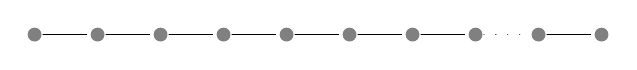
\begin{tikzpicture}[scale=0.8,->,>=stealth',shorten >=1pt,auto,node distance=3cm,
    thick,main node/.style={circle,draw,font=\footnotesize}, small node/.style={circle,font=\footnotesize,inner sep=0pt,minimum size=5pt}]   
    \begin{scope}     
%     \node[inner sep=0pt] (robot) at (4,5)
%     {\includegraphics[width=.02\textwidth,right]{robot1.jpg} };
      \node[small node,fill=gray] (a) at (1,5) {};
      \node[small node,fill=gray] (b) at (2,5) {};
      \node[small node,fill=gray] (c) at (3,5) {};
      \node[small node,fill=gray] (d) at (4,5) {};
      \node[small node,fill=gray] (e) at (5,5) {};    
      \node[small node,fill=gray] (f) at (6,5) {};
      \node[small node,fill=gray] (g) at (7,5) {};
      \node[small node,fill=gray] (h) at (8,5) {};
      \node[small node,fill=gray] (i) at (9,5) {};
      \node[small node,fill=gray] (j) at (10,5) {}; 
      \path[-,line width=0.3pt] (a) edge (b);
      \path[-,line width=0.3pt] (b) edge (c);
      \path[-,line width=0.3pt] (c) edge (d);
      \path[-,line width=0.3pt] (d) edge (e);
      \path[-,line width=0.3pt] (e) edge (f);
      \path[-,line width=0.3pt] (f) edge (g);
      \path[-,line width=0.3pt] (g) edge (h);
      \path[-,line width=0.3pt, loosely dotted] (h) edge (i);
      \path[-,line width=0.3pt] (i) edge (j);
    \end{scope}
  \end{tikzpicture} 
  & $n$ nodes\\ 
    &  \\
    &  \\
    &  \\
    &  \\
    &  \\
\end{tabular}
\end{frame}
\miniframesoff
\begin{frame}{Model} %%% MODEL 1 %%%
\begin{tabular}{rl}
  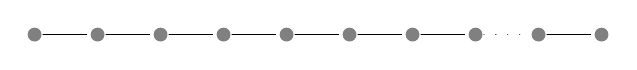
\begin{tikzpicture}[scale=0.8,->,>=stealth',shorten >=1pt,auto,node distance=3cm,
    thick,main node/.style={circle,draw,font=\footnotesize}, small node/.style={circle,font=\footnotesize,inner sep=0pt,minimum size=5pt}]   
    \begin{scope}     
%     \node[inner sep=0pt] (robot) at (4,5)
%     {\includegraphics[width=.02\textwidth,right]{robot1.jpg} };
      \node[small node,fill=gray] (a) at (1,5) {};
      \node[small node,fill=gray] (b) at (2,5) {};
      \node[small node,fill=gray] (c) at (3,5) {};
      \node[small node,fill=gray] (d) at (4,5) {};
      \node[small node,fill=gray] (e) at (5,5) {};    
      \node[small node,fill=gray] (f) at (6,5) {};
      \node[small node,fill=gray] (g) at (7,5) {};
      \node[small node,fill=gray] (h) at (8,5) {};
      \node[small node,fill=gray] (i) at (9,5) {};
      \node[small node,fill=gray] (j) at (10,5) {}; 
      \path[-,line width=0.3pt] (a) edge (b);
      \path[-,line width=0.3pt] (b) edge (c);
      \path[-,line width=0.3pt] (c) edge (d);
      \path[-,line width=0.3pt] (d) edge (e);
      \path[-,line width=0.3pt] (e) edge (f);
      \path[-,line width=0.3pt] (f) edge (g);
      \path[-,line width=0.3pt] (g) edge (h);
      \path[-,line width=0.3pt, loosely dotted] (h) edge (i);
      \path[-,line width=0.3pt] (i) edge (j);
    \end{scope}
  \end{tikzpicture} 
  & $n$ nodes\\ 
    &  \\
    &  \\
    &  \\
    &  \\
    &  \\
\end{tabular}
\end{frame}

\begin{frame}{Model} %%% MODEL 2 %%%
\begin{tabular}{rl}
  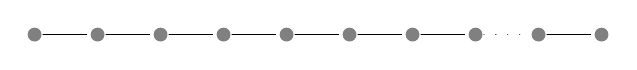
\begin{tikzpicture}[scale=0.8,->,>=stealth',shorten >=1pt,auto,node distance=3cm,
    thick,main node/.style={circle,draw,font=\footnotesize}, small node/.style={circle,font=\footnotesize,inner sep=0pt,minimum size=5pt}]   
    \begin{scope}     
%     \node[inner sep=0pt] (robot) at (4,5)
%     {\includegraphics[width=.02\textwidth,right]{robot1.jpg} };
      \node[small node,fill=gray] (a) at (1,5) {};
      \node[small node,fill=gray] (b) at (2,5) {};
      \node[small node,fill=gray] (c) at (3,5) {};
      \node[small node,fill=gray] (d) at (4,5) {};
      \node[small node,fill=gray] (e) at (5,5) {};    
      \node[small node,fill=gray] (f) at (6,5) {};
      \node[small node,fill=gray] (g) at (7,5) {};
      \node[small node,fill=gray] (h) at (8,5) {};
      \node[small node,fill=gray] (i) at (9,5) {};
      \node[small node,fill=gray] (j) at (10,5) {}; 
      \path[-,line width=0.3pt] (a) edge (b);
      \path[-,line width=0.3pt] (b) edge (c);
      \path[-,line width=0.3pt] (c) edge (d);
      \path[-,line width=0.3pt] (d) edge (e);
      \path[-,line width=0.3pt] (e) edge (f);
      \path[-,line width=0.3pt] (f) edge (g);
      \path[-,line width=0.3pt] (g) edge (h);
      \path[-,line width=0.3pt, loosely dotted] (h) edge (i);
      \path[-,line width=0.3pt] (i) edge (j);
    \end{scope}
  \end{tikzpicture} 
  & $n$ nodes\\ 
      &  \\
  
\includegraphics[width=.05\textwidth,right]{robot1.jpg} 
  
\includegraphics[width=.05\textwidth,right]{robot1.jpg} 
  
\includegraphics[width=.05\textwidth,right]{robot1.jpg}  
  
\includegraphics[width=.05\textwidth,right]{robot1.jpg} 
  & $k$ robots\\
    &  \\
    &  \\
    &  \\
\end{tabular}
\end{frame}

\begin{frame}{Model} %%% MODEL 3 %%%
\begin{tabular}{rl}
  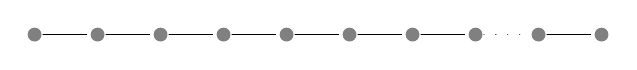
\begin{tikzpicture}[scale=0.8,->,>=stealth',shorten >=1pt,auto,node distance=3cm,
    thick,main node/.style={circle,draw,font=\footnotesize}, small node/.style={circle,font=\footnotesize,inner sep=0pt,minimum size=5pt}]   
    \begin{scope}     
%     \node[inner sep=0pt] (robot) at (4,5)
%     {\includegraphics[width=.02\textwidth,right]{robot1.jpg} };
      \node[small node,fill=gray] (a) at (1,5) {};
      \node[small node,fill=gray] (b) at (2,5) {};
      \node[small node,fill=gray] (c) at (3,5) {};
      \node[small node,fill=gray] (d) at (4,5) {};
      \node[small node,fill=gray] (e) at (5,5) {};    
      \node[small node,fill=gray] (f) at (6,5) {};
      \node[small node,fill=gray] (g) at (7,5) {};
      \node[small node,fill=gray] (h) at (8,5) {};
      \node[small node,fill=gray] (i) at (9,5) {};
      \node[small node,fill=gray] (j) at (10,5) {}; 
      \path[-,line width=0.3pt] (a) edge (b);
      \path[-,line width=0.3pt] (b) edge (c);
      \path[-,line width=0.3pt] (c) edge (d);
      \path[-,line width=0.3pt] (d) edge (e);
      \path[-,line width=0.3pt] (e) edge (f);
      \path[-,line width=0.3pt] (f) edge (g);
      \path[-,line width=0.3pt] (g) edge (h);
      \path[-,line width=0.3pt, loosely dotted] (h) edge (i);
      \path[-,line width=0.3pt] (i) edge (j);
    \end{scope}
  \end{tikzpicture} 
  & $n$ nodes\\ 
      &  \\
  
\includegraphics[width=.05\textwidth,right]{robot1.jpg} 
  
\includegraphics[width=.05\textwidth,right]{robot1.jpg} 
  
\includegraphics[width=.05\textwidth,right]{robot1.jpg}  
  
\includegraphics[width=.05\textwidth,right]{robot1.jpg} 
  & $k$ robots\\
    &  \\
        &  \\
    \begin{tikzpicture}[scale=0.8,->,>=stealth',shorten >=1pt,auto,node distance=3cm,
    thick,main node/.style={circle,draw,font=\footnotesize}, small node/.style={circle,font=\footnotesize,inner sep=0pt,minimum size=5pt}]   
    \begin{scope}     
%     \node[inner sep=0pt] (robot) at (4,5)
%     {
\includegraphics[width=.02\textwidth,right]{robot1.jpg} };
      \node[small node,fill=gray] (a) at (1,5) {};
      \node[inner sep=0pt]  (b) at (2,5) {
\includegraphics[width=.03\textwidth,right]{robot1.jpg}};
      \node[small node,fill=gray] (c) at (3,5) {};
      \node[inner sep=0pt]  (d) at (4,5) {
\includegraphics[width=.03\textwidth,right]{robot1.jpg}};
      \node[inner sep=0pt]  (e) at (5,5) {
\includegraphics[width=.03\textwidth,right]{robot1.jpg}};    
      \node[small node,fill=gray] (f) at (6,5) {};
      \node[inner sep=0pt]  (g) at (7,5) {
\includegraphics[width=.03\textwidth,right]{robot1.jpg}};
      \node[small node,fill=gray] (h) at (8,5) {};
      \node[small node,fill=gray] (i) at (9,5) {};
      \node[small node,fill=gray] (j) at (10,5) {}; 
      
%       \node[inner sep=0pt]   at (2,5.5) {
\includegraphics[width=.03\textwidth,right]{robot1.jpg}};
%       \node[inner sep=0pt]   at (5,5.5) {
\includegraphics[width=.03\textwidth,right]{robot1.jpg}};
%       \node[inner sep=0pt]   at (5,6) {
\includegraphics[width=.03\textwidth,right]{robot1.jpg}};
      \path[-,line width=0.3pt] (a) edge (b);
      \path[-,line width=0.3pt] (b) edge (c);
      \path[-,line width=0.3pt] (c) edge (d);
      \path[-,line width=0.3pt] (d) edge (e);
      \path[-,line width=0.3pt] (e) edge (f);
      \path[-,line width=0.3pt] (f) edge (g);
      \path[-,line width=0.3pt] (g) edge (h);
      \path[-,line width=0.3pt, loosely dotted] (h) edge (i);
      \path[-,line width=0.3pt] (i) edge (j);
    \end{scope}
  \end{tikzpicture}
  & \\
\end{tabular}
\end{frame}

\begin{frame}{Model} %%% MODEL 4 %%%
\begin{tabular}{rl}
  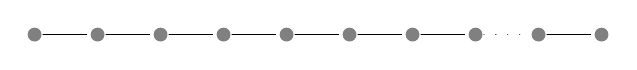
\begin{tikzpicture}[scale=0.8,->,>=stealth',shorten >=1pt,auto,node distance=3cm,
    thick,main node/.style={circle,draw,font=\footnotesize}, small node/.style={circle,font=\footnotesize,inner sep=0pt,minimum size=5pt}]   
    \begin{scope}     
%     \node[inner sep=0pt] (robot) at (4,5)
%     {\includegraphics[width=.02\textwidth,right]{robot1.jpg} };
      \node[small node,fill=gray] (a) at (1,5) {};
      \node[small node,fill=gray] (b) at (2,5) {};
      \node[small node,fill=gray] (c) at (3,5) {};
      \node[small node,fill=gray] (d) at (4,5) {};
      \node[small node,fill=gray] (e) at (5,5) {};    
      \node[small node,fill=gray] (f) at (6,5) {};
      \node[small node,fill=gray] (g) at (7,5) {};
      \node[small node,fill=gray] (h) at (8,5) {};
      \node[small node,fill=gray] (i) at (9,5) {};
      \node[small node,fill=gray] (j) at (10,5) {}; 
      \path[-,line width=0.3pt] (a) edge (b);
      \path[-,line width=0.3pt] (b) edge (c);
      \path[-,line width=0.3pt] (c) edge (d);
      \path[-,line width=0.3pt] (d) edge (e);
      \path[-,line width=0.3pt] (e) edge (f);
      \path[-,line width=0.3pt] (f) edge (g);
      \path[-,line width=0.3pt] (g) edge (h);
      \path[-,line width=0.3pt, loosely dotted] (h) edge (i);
      \path[-,line width=0.3pt] (i) edge (j);
    \end{scope}
  \end{tikzpicture} 
  & $n$ nodes\\ 
      &  \\
  
\includegraphics[width=.05\textwidth,right]{robot1.jpg} 
  
\includegraphics[width=.05\textwidth,right]{robot1.jpg} 
  
\includegraphics[width=.05\textwidth,right]{robot1.jpg}  
  
\includegraphics[width=.05\textwidth,right]{robot1.jpg} 
  & $k$ robots\\
    &  \\
        &  \\
    \begin{tikzpicture}[scale=0.8,->,>=stealth',shorten >=1pt,auto,node distance=3cm,
    thick,main node/.style={circle,draw,font=\footnotesize}, small node/.style={circle,font=\footnotesize,inner sep=0pt,minimum size=5pt}]   
    \begin{scope}     
     \node[inner sep=0pt] (robot) at (4,5)
     {
\includegraphics[width=.02\textwidth,right]{robot1.jpg} };
      \node[small node,fill=gray] (a) at (1,5) {};
      \node[inner sep=0pt]  (b) at (2,5) {
\includegraphics[width=.03\textwidth,right]{robot1.jpg}};
      \node[small node,fill=gray] (c) at (3,5) {};
      \node[inner sep=0pt]  (d) at (4,5) {
\includegraphics[width=.03\textwidth,right]{robot1.jpg}};
      \node[inner sep=0pt]  (e) at (5,5) {
\includegraphics[width=.03\textwidth,right]{robot1.jpg}};    
      \node[small node,fill=gray] (f) at (6,5) {};
      \node[inner sep=0pt]  (g) at (7,5) {
\includegraphics[width=.03\textwidth,right]{robot1.jpg}};
      \node[small node,fill=gray] (h) at (8,5) {};
      \node[small node,fill=gray] (i) at (9,5) {};
      \node[small node,fill=gray] (j) at (10,5) {}; 
      
       \node[inner sep=0pt]   at (2,5.5) {
\includegraphics[width=.03\textwidth,right]{robot1.jpg}};
       \node[inner sep=0pt]   at (5,5.5) {
\includegraphics[width=.03\textwidth,right]{robot1.jpg}};
       \node[inner sep=0pt]   at (5,6) {
\includegraphics[width=.03\textwidth,right]{robot1.jpg}};
      \path[-,line width=0.3pt] (a) edge (b);
      \path[-,line width=0.3pt] (b) edge (c);
      \path[-,line width=0.3pt] (c) edge (d);
      \path[-,line width=0.3pt] (d) edge (e);
      \path[-,line width=0.3pt] (e) edge (f);
      \path[-,line width=0.3pt] (f) edge (g);
      \path[-,line width=0.3pt] (g) edge (h);
      \path[-,line width=0.3pt, loosely dotted] (h) edge (i);
      \path[-,line width=0.3pt] (i) edge (j);
    \end{scope}
  \end{tikzpicture}
  & \\
\end{tabular}
\end{frame}
\miniframeson
\begin{frame}{Look}
%\resizebox{<horizontal size>}{<vertical size>}{%
    \begin{tikzpicture}[scale=0.8,->,>=stealth',shorten >=1pt,auto,node distance=3cm,
    thick,main node/.style={circle,draw,font=\footnotesize}, small node/.style={circle,font=\footnotesize,inner sep=0pt,minimum size=5pt}]   

    \begin{scope}%[xshift=10cm]
      \node[small node,fill=gray] (b) at (2,5) {};
      \node[inner sep=0pt]  (c) at (4,5) {
\includegraphics[width=.03\textwidth,right]{robot1.jpg}};
      \node[inner sep=0pt]  (d) at (6,5) {
\includegraphics[width=.03\textwidth,right]{robot1.jpg}};
      \node[small node,fill=gray] (e) at (8,5) {};    
      \node[inner sep=0pt]  (f) at (10,5) {
\includegraphics[width=.03\textwidth,right]{robot1.jpg}};
      \node[inner sep=0pt] at (10,5.5) {
\includegraphics[width=.03\textwidth,right]{robot1.jpg}};
      \node[small node,fill=gray] (i) at (12,5) {};
      \node[small node,fill=gray] (j) at (14,5) {};
      \path[-,line width=0.3pt] (b) edge (c);
      \path[-,line width=0.3pt] (c) edge (d);
      \path[-,line width=0.3pt] (d) edge (e);
      \path[-,line width=0.3pt] (e) edge (f);
      \path[-,line width=0.3pt] (f) edge (i);
      \path[-,line width=0.3pt] (i) edge (j);
      \path[-,line width=0.3pt, color=pink] (d) edge [bend right,-] (7.2,6.8);
       
   \end{scope}
   \begin{scope}[scale=0.4, xshift=12cm,yshift=12cm]
      \node[small node,fill=gray] (b) at (2,5) {};
      \node[small node,fill=gray] (c) at (4,5) {};
      %\node[inner sep=0pt]  (d) at (6,5) {
\includegraphics[width=.03\textwidth,right]{robot1.jpg}};
      \node[small node,fill=pink] (d) at (6,5) {};
      \node[small node,fill=gray] (e) at (8,5) {};    
      \node[small node,fill=gray] (f) at (10,5) {};
      \node[small node,fill=gray] (i) at (12,5) {};
      \node[small node,fill=gray] (j) at (14,5) {};
      \path[-,line width=0.3pt] (b) edge (c);
      \path[-,line width=0.3pt] (c) edge (d);
      \path[-,line width=0.3pt] (d) edge (e);
      \path[-,line width=0.3pt] (e) edge (f);
      \path[-,line width=0.3pt] (f) edge (i);
      \path[-,line width=0.3pt] (i) edge (j);
    \end{scope}
  \end{tikzpicture}
\end{frame}
\miniframesoff
\begin{frame}{Look}

%\resizebox{<horizontal size>}{<vertical size>}{%
    \begin{tikzpicture}[scale=0.8,->,>=stealth',shorten >=1pt,auto,node distance=3cm,
    thick,main node/.style={circle,draw,font=\footnotesize}, small node/.style={circle,font=\footnotesize,inner sep=0pt,minimum size=5pt}]   

    \begin{scope}%[xshift=10cm]
      \node[small node,fill=gray] (b) at (2,5) {};
      \node[inner sep=0pt]  (c) at (4,5) {
\includegraphics[width=.03\textwidth,right]{robot1.jpg}};
      \node[inner sep=0pt]  (d) at (6,5) {
\includegraphics[width=.03\textwidth,right]{robot1.jpg}};
      \node[small node,fill=gray] (e) at (8,5) {};    
      \node[inner sep=0pt]  (f) at (10,5) {
\includegraphics[width=.03\textwidth,right]{robot1.jpg}};
      \node[inner sep=0pt] at (10,5.5) {
\includegraphics[width=.03\textwidth,right]{robot1.jpg}};
      \node[small node,fill=gray] (i) at (12,5) {};
      \node[small node,fill=gray] (j) at (14,5) {};
      \path[-,line width=0.3pt] (b) edge (c);
      \path[-,line width=0.3pt] (c) edge (d);
      \path[-,line width=0.3pt] (d) edge (e);
      \path[-,line width=0.3pt] (e) edge (f);
      \path[-,line width=0.3pt] (f) edge (i);
      \path[-,line width=0.3pt] (i) edge (j);

      \path[-,line width=0.3pt, color=pink] (d) edge [bend right,-] (7.2,6.8);
% 
%       
    \end{scope}
        \begin{scope}[scale=0.4, xshift=12cm,yshift=12cm]
      \node[small node,fill=gray] (b) at (2,5) {};
      \node[small node,fill=black] (c) at (4,5) {};
      %\node[inner sep=0pt]  (d) at (6,5) {
\includegraphics[width=.03\textwidth,right]{robot1.jpg}};
      \node[small node,fill=pink] (d) at (6,5) {};
      \node[small node,fill=gray] (e) at (8,5) {};    
      \node[diamond, fill=black]  (f) at (10,5) {};
      \node[small node,fill=gray] (i) at (12,5) {};
      \node[small node,fill=gray] (j) at (14,5) {};
      \path[-,line width=0.3pt] (b) edge (c);
      \path[-,line width=0.3pt] (c) edge (d);
      \path[-,line width=0.3pt] (d) edge (e);
      \path[-,line width=0.3pt] (e) edge (f);
      \path[-,line width=0.3pt] (f) edge (i);
      \path[-,line width=0.3pt] (i) edge (j);

    \end{scope}
  \end{tikzpicture}
\end{frame}

\begin{frame}{Look} %%% LOOK 2,5 %%%

%\resizebox{<horizontal size>}{<vertical size>}{%
    \begin{tikzpicture}[scale=0.8,->,>=stealth',shorten >=1pt,auto,node distance=3cm,
    thick,main node/.style={circle,draw,font=\footnotesize}, small node/.style={circle,font=\footnotesize,inner sep=0pt,minimum size=5pt}]   

    \begin{scope}%[xshift=10cm]
      \node[small node,fill=gray] (b) at (2,5) {};
      \node[inner sep=0pt]  (c) at (4,5) {
\includegraphics[width=.03\textwidth,right]{robot1.jpg}};
      \node[inner sep=0pt]  (d) at (6,5) {
\includegraphics[width=.03\textwidth,right]{robot1.jpg}};
      \node[small node,fill=gray] (e) at (8,5) {};    
      \node[inner sep=0pt]  (f) at (10,5) {
\includegraphics[width=.03\textwidth,right]{robot1.jpg}};
      \node[inner sep=0pt] at (10,5.5) {
\includegraphics[width=.03\textwidth,right]{robot1.jpg}};
      \node[small node,fill=gray] (i) at (12,5) {};
      \node[small node,fill=gray] (j) at (14,5) {};
      \path[-,line width=0.3pt] (b) edge (c);
      \path[-,line width=0.3pt] (c) edge (d);
      \path[-,line width=0.3pt] (d) edge (e);
      \path[-,line width=0.3pt] (e) edge (f);
      \path[-,line width=0.3pt] (f) edge (i);
      \path[-,line width=0.3pt] (i) edge (j);

      \path[-,line width=0.3pt, color=pink] (f) edge [bend left,-] (8.8,6.8);
 
       
    \end{scope}
    \begin{scope}[scale=0.4, xshift=12cm,yshift=12cm]
      \node[small node,fill=gray] (b) at (2,5) {};
      \node[small node,fill=gray] (c) at (4,5) {};
      %\node[inner sep=0pt]  (d) at (6,5) {
\includegraphics[width=.03\textwidth,right]{robot1.jpg}};
       \node[small node,fill=gray] (d) at (6,5) {};
       \node[small node,fill=gray] (e) at (8,5) {};  
      \node[diamond, fill=gray]  (f) at (10,5) {};
      \node[small node,fill=pink] at (10,5) {};
      \node[small node,fill=gray] (i) at (12,5) {};
      \node[small node,fill=gray] (j) at (14,5) {};
      \path[-,line width=0.3pt] (b) edge (c);
      \path[-,line width=0.3pt] (c) edge (d);
      \path[-,line width=0.3pt] (d) edge (e);
      \path[-,line width=0.3pt] (e) edge (f);
      \path[-,line width=0.3pt] (f) edge (i);
      \path[-,line width=0.3pt] (i) edge (j);

    \end{scope}
  \end{tikzpicture}
\end{frame}

\begin{frame}{Look} %%% LOOK 3 %%%

%\resizebox{<horizontal size>}{<vertical size>}{%
    \begin{tikzpicture}[scale=0.8,->,>=stealth',shorten >=1pt,auto,node distance=3cm,
    thick,main node/.style={circle,draw,font=\footnotesize}, small node/.style={circle,font=\footnotesize,inner sep=0pt,minimum size=5pt}]   

    \begin{scope}%[xshift=10cm]
      \node[small node,fill=gray] (b) at (2,5) {};
      \node[inner sep=0pt]  (c) at (4,5) {\includegraphics[width=.03\textwidth,right]{robot1.jpg}};
      \node[inner sep=0pt]  (d) at (6,5) {\includegraphics[width=.03\textwidth,right]{robot1.jpg}};
      \node[small node,fill=gray] (e) at (8,5) {};    
      \node[inner sep=0pt]  (f) at (10,5) {\includegraphics[width=.03\textwidth,right]{robot1.jpg}};
      \node[inner sep=0pt] at (10,5.5) {\includegraphics[width=.03\textwidth,right]{robot1.jpg}};
      \node[small node,fill=gray] (i) at (12,5) {};
      \node[small node,fill=gray] (j) at (14,5) {};
      \path[-,line width=0.3pt] (b) edge (c);
      \path[-,line width=0.3pt] (c) edge (d);
      \path[-,line width=0.3pt] (d) edge (e);
      \path[-,line width=0.3pt] (e) edge (f);
      \path[-,line width=0.3pt] (f) edge (i);
      \path[-,line width=0.3pt] (i) edge (j);

      \path[-,line width=0.3pt, color=pink] (f) edge [bend left,-] (8.8,6.8);
 
       
    \end{scope}
    \begin{scope}[scale=0.4, xshift=12cm,yshift=12cm]
      \node[small node,fill=gray] (b) at (2,5) {};
      \node[small node,fill=black] (c) at (4,5) {};
      %\node[inner sep=0pt]  (d) at (6,5) {\includegraphics[width=.03\textwidth,right]{robot1.jpg}};
       \node[small node,fill=black] (d) at (6,5) {};
       \node[small node,fill=gray] (e) at (8,5) {};    

      \node[diamond, fill=pink]  (f) at (10,5) {};
      \node[small node,fill=gray] (i) at (12,5) {};
      \node[small node,fill=gray] (j) at (14,5) {};
       \path[-,line width=0.3pt] (b) edge (c);
       \path[-,line width=0.3pt] (c) edge (d);
       \path[-,line width=0.3pt] (d) edge (e);
      \path[-,line width=0.3pt] (e) edge (f);
      \path[-,line width=0.3pt] (f) edge (i);
      \path[-,line width=0.3pt] (i) edge (j);

    \end{scope}
  \end{tikzpicture}
\end{frame}

\miniframeson
\begin{frame}{Look} %%% CYCLE 1 %%%

    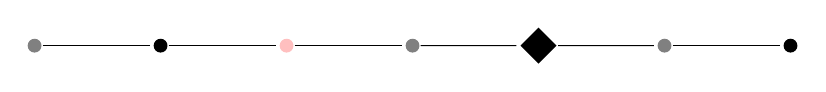
\begin{tikzpicture}[scale=0.8,->,>=stealth',shorten >=1pt,auto,node distance=3cm,
    thick,main node/.style={circle,draw,font=\footnotesize}, small node/.style={circle,font=\footnotesize,inner sep=0pt,minimum size=5pt}]   
    \begin{scope}%[xshift=10cm]
     \node[small node,fill=gray] (b) at (2,5) {};
      \node[small node,fill=black] (c) at (4,5) {};
      %\node[inner sep=0pt]  (d) at (6,5) {\includegraphics[width=.03\textwidth,right]{robot1.jpg}};
       \node[small node,fill=pink] (d) at (6,5) {};
       \node[small node,fill=gray] (e) at (8,5) {};    

      \node[diamond, fill=black]  (f) at (10,5) {};
      \node[small node,fill=gray] (i) at (12,5) {};
      \node[small node,fill=black] (j) at (14,5) {};
       \path[-,line width=0.3pt] (b) edge (c);
       \path[-,line width=0.3pt] (c) edge (d);
       \path[-,line width=0.3pt] (d) edge (e);
      \path[-,line width=0.3pt] (e) edge (f);
      \path[-,line width=0.3pt] (f) edge (i);
      \path[-,line width=0.3pt] (i) edge (j);
      %\path[-,line width=0.3pt, color=pink] (f) edge [bend left,-] (8.8,6.8);       

    \end{scope}
  \end{tikzpicture}
\end{frame}
\miniframesoff
\begin{frame}{Compute} %%% CYCLE 5 %%%

    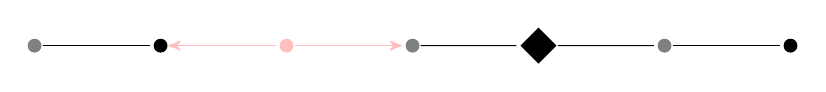
\begin{tikzpicture}[scale=0.8,->,>=stealth',shorten >=1pt,auto,node distance=3cm,
    thick,main node/.style={circle,draw,font=\footnotesize}, small node/.style={circle,font=\footnotesize,inner sep=0pt,minimum size=5pt}]   
    \begin{scope}%[xshift=10cm]
     \node[small node,fill=gray] (b) at (2,5) {};
      \node[small node,fill=black] (c) at (4,5) {};
      %\node[inner sep=0pt]  (d) at (6,5) {\includegraphics[width=.03\textwidth,right]{robot1.jpg}};
       \node[small node,fill=pink] (d) at (6,5) {};
       \node[small node,fill=gray] (e) at (8,5) {};    

      \node[diamond, fill=black]  (f) at (10,5) {};
      \node[small node,fill=gray] (i) at (12,5) {};
      \node[small node,fill=black] (j) at (14,5) {};
      \path[-,line width=0.3pt] (b) edge (c);
       \path[<-,line width=0.6pt, color=pink] (c) edge (d);
       \path[->,line width=0.6pt, color=pink] (d) edge (e);
      \path[-,line width=0.3pt] (e) edge (f);
      \path[-,line width=0.3pt] (f) edge (i);
      \path[-,line width=0.3pt] (i) edge (j);
      %\path[-,line width=0.3pt, color=pink] (f) edge [bend left,-] (8.8,6.8);       

    \end{scope}
  \end{tikzpicture}
\end{frame}

\begin{frame}{Move} %%% CYCLE 1 %%%

    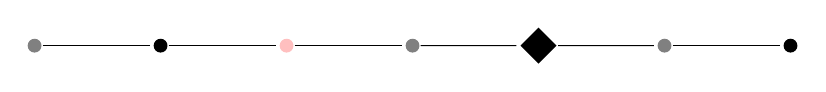
\begin{tikzpicture}[scale=0.8,->,>=stealth',shorten >=1pt,auto,node distance=3cm,
    thick,main node/.style={circle,draw,font=\footnotesize}, small node/.style={circle,font=\footnotesize,inner sep=0pt,minimum size=5pt}]   
    \begin{scope}%[xshift=10cm]
     \node[small node,fill=gray] (b) at (2,5) {};
      \node[small node,fill=black] (c) at (4,5) {};
      %\node[inner sep=0pt]  (d) at (6,5) {\includegraphics[width=.03\textwidth,right]{robot1.jpg}};
       \node[small node,fill=pink] (d) at (6,5) {};
       \node[small node,fill=gray] (e) at (8,5) {};    

      \node[diamond, fill=black]  (f) at (10,5) {};
      \node[small node,fill=gray] (i) at (12,5) {};
      \node[small node,fill=black] (j) at (14,5) {};
       \path[-,line width=0.3pt] (b) edge (c);
       \path[-,line width=0.3pt] (c) edge (d);
       \path[-,line width=0.3pt] (d) edge (e);
      \path[-,line width=0.3pt] (e) edge (f);
      \path[-,line width=0.3pt] (f) edge (i);
      \path[-,line width=0.3pt] (i) edge (j);
      %\path[-,line width=0.3pt, color=pink] (f) edge [bend left,-] (8.8,6.8);       

    \end{scope}
  \end{tikzpicture}
\end{frame}

\begin{frame}{Move} %%% CYCLE 3 %%%

    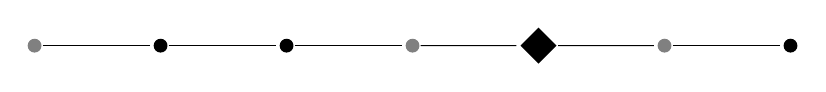
\begin{tikzpicture}[scale=0.8,->,>=stealth',shorten >=1pt,auto,node distance=3cm,
    thick,main node/.style={circle,draw,font=\footnotesize}, small node/.style={circle,font=\footnotesize,inner sep=0pt,minimum size=5pt}]   
    \begin{scope}%[xshift=10cm]
     \node[small node,fill=gray] (b) at (2,5) {};
      \node[small node,fill=black] (c) at (4,5) {};
      %\node[inner sep=0pt]  (d) at (6,5) {\includegraphics[width=.03\textwidth,right]{robot1.jpg}};
       \node[small node,fill=black] (d) at (6,5) {};
       \node[small node,fill=gray] (e) at (8,5) {};    

      \node[diamond, fill=black]  (f) at (10,5) {};
      \node[small node,fill=gray] (i) at (12,5) {};
      \node[small node,fill=black] (j) at (14,5) {};
       \path[-,line width=0.3pt] (b) edge (c);
       \path[-,line width=0.3pt] (c) edge (d);
       \path[-,line width=0.3pt] (d) edge (e);
      \path[-,line width=0.3pt] (e) edge (f);
      \path[-,line width=0.3pt] (f) edge (i);
      \path[-,line width=0.3pt] (i) edge (j);
      %\path[-,line width=0.3pt, color=pink] (f) edge [bend left,-] (8.8,6.8);       

    \end{scope}
  \end{tikzpicture}
\end{frame}

\begin{frame}{Look} %%% CYCLE 4 %%%

    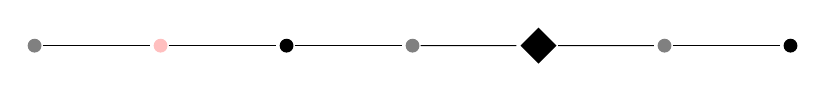
\begin{tikzpicture}[scale=0.8,->,>=stealth',shorten >=1pt,auto,node distance=3cm,
    thick,main node/.style={circle,draw,font=\footnotesize}, small node/.style={circle,font=\footnotesize,inner sep=0pt,minimum size=5pt}]   
    \begin{scope}%[xshift=10cm]
     \node[small node,fill=gray] (b) at (2,5) {};
      \node[small node,fill=pink] (c) at (4,5) {};
      %\node[inner sep=0pt]  (d) at (6,5) {\includegraphics[width=.03\textwidth,right]{robot1.jpg}};
       \node[small node,fill=black] (d) at (6,5) {};
       \node[small node,fill=gray] (e) at (8,5) {};    

      \node[diamond, fill=black]  (f) at (10,5) {};
      \node[small node,fill=gray] (i) at (12,5) {};
      \node[small node,fill=black] (j) at (14,5) {};
       \path[-,line width=0.3pt] (b) edge (c);
       \path[-,line width=0.3pt] (c) edge (d);
       \path[-,line width=0.3pt] (d) edge (e);
      \path[-,line width=0.3pt] (e) edge (f);
      \path[-,line width=0.3pt] (f) edge (i);
      \path[-,line width=0.3pt] (i) edge (j);
      %\path[-,line width=0.3pt, color=pink] (f) edge [bend left,-] (8.8,6.8);       

    \end{scope}
  \end{tikzpicture}
\end{frame}

\begin{frame}{Compute} %%% CYCLE 5 %%%

    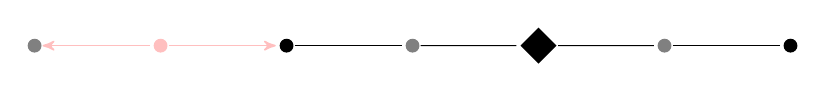
\begin{tikzpicture}[scale=0.8,->,>=stealth',shorten >=1pt,auto,node distance=3cm,
    thick,main node/.style={circle,draw,font=\footnotesize}, small node/.style={circle,font=\footnotesize,inner sep=0pt,minimum size=5pt}]   
    \begin{scope}%[xshift=10cm]
     \node[small node,fill=gray] (b) at (2,5) {};
      \node[small node,fill=pink] (c) at (4,5) {};
      %\node[inner sep=0pt]  (d) at (6,5) {\includegraphics[width=.03\textwidth,right]{robot1.jpg}};
       \node[small node,fill=black] (d) at (6,5) {};
       \node[small node,fill=gray] (e) at (8,5) {};    

      \node[diamond, fill=black]  (f) at (10,5) {};
      \node[small node,fill=gray] (i) at (12,5) {};
      \node[small node,fill=black] (j) at (14,5) {};
       \path[<-,line width=0.6pt, color=pink] (b) edge (c);
       \path[->,line width=0.6pt, color=pink] (c) edge (d);
       \path[-,line width=0.3pt]  (d) edge (e);
      \path[-,line width=0.3pt] (e) edge (f);
      \path[-,line width=0.3pt] (f) edge (i);
      \path[-,line width=0.3pt] (i) edge (j);
      %\path[-,line width=0.3pt, color=pink] (f) edge [bend left,-] (8.8,6.8);       

    \end{scope}
  \end{tikzpicture}
\end{frame}

\begin{frame}{Move} %%% CYCLE 6 %%%

    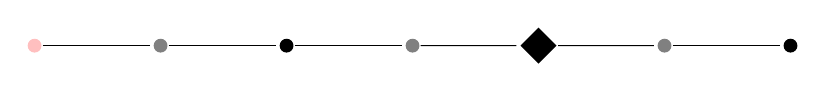
\begin{tikzpicture}[scale=0.8,->,>=stealth',shorten >=1pt,auto,node distance=3cm,
    thick,main node/.style={circle,draw,font=\footnotesize}, small node/.style={circle,font=\footnotesize,inner sep=0pt,minimum size=5pt}]   
    \begin{scope}%[xshift=10cm]
     \node[small node,fill=pink] (b) at (2,5) {};
      \node[small node,fill=gray] (c) at (4,5) {};
      %\node[inner sep=0pt]  (d) at (6,5) {\includegraphics[width=.03\textwidth,right]{robot1.jpg}};
       \node[small node,fill=black] (d) at (6,5) {};
       \node[small node,fill=gray] (e) at (8,5) {};    

      \node[diamond, fill=black]  (f) at (10,5) {};
      \node[small node,fill=gray] (i) at (12,5) {};
      \node[small node,fill=black] (j) at (14,5) {};
       \path[-,line width=0.3pt] (b) edge (c);
       \path[-,line width=0.3pt] (c) edge (d);
       \path[-,line width=0.3pt] (d) edge (e);
      \path[-,line width=0.3pt] (e) edge (f);
      \path[-,line width=0.3pt] (f) edge (i);
      \path[-,line width=0.3pt] (i) edge (j);
      %\path[-,line width=0.3pt, color=pink] (f) edge [bend left,-] (8.8,6.8);       

    \end{scope}
  \end{tikzpicture}
\end{frame}

\begin{frame}{Move} %%% CYCLE 7 %%%

    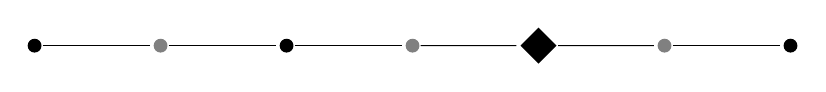
\begin{tikzpicture}[scale=0.8,->,>=stealth',shorten >=1pt,auto,node distance=3cm,
    thick,main node/.style={circle,draw,font=\footnotesize}, small node/.style={circle,font=\footnotesize,inner sep=0pt,minimum size=5pt}]   
    \begin{scope}%[xshift=10cm]
     \node[small node,fill=black] (b) at (2,5) {};
      \node[small node,fill=gray] (c) at (4,5) {};
      %\node[inner sep=0pt]  (d) at (6,5) {\includegraphics[width=.03\textwidth,right]{robot1.jpg}};
       \node[small node,fill=black] (d) at (6,5) {};
       \node[small node,fill=gray] (e) at (8,5) {};    

      \node[diamond, fill=black]  (f) at (10,5) {};
      \node[small node,fill=gray] (i) at (12,5) {};
      \node[small node,fill=black] (j) at (14,5) {};
       \path[-,line width=0.3pt] (b) edge (c);
       \path[-,line width=0.3pt] (c) edge (d);
       \path[-,line width=0.3pt] (d) edge (e);
      \path[-,line width=0.3pt] (e) edge (f);
      \path[-,line width=0.3pt] (f) edge (i);
      \path[-,line width=0.3pt] (i) edge (j);
      %\path[-,line width=0.3pt, color=pink] (f) edge [bend left,-] (8.8,6.8);       

    \end{scope}
  \end{tikzpicture}
\end{frame}
\miniframeson
\begin{frame}{Robots: Asynchronous} %%% CYCLE 7 %%%

    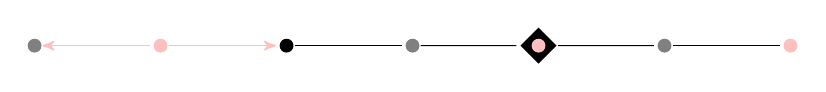
\begin{tikzpicture}[scale=0.8,->,>=stealth',shorten >=1pt,auto,node distance=3cm,
    thick,main node/.style={circle,draw,font=\footnotesize}, small node/.style={circle,font=\footnotesize,inner sep=0pt,minimum size=5pt}]   
   \begin{scope}%[xshift=10cm]
     \node[small node,fill=gray] (b) at (2,5) {};
      \node[small node,fill=pink] (c) at (4,5) {};
      %\node[inner sep=0pt]  (d) at (6,5) {\includegraphics[width=.03\textwidth,right]{robot1.jpg}};
       \node[small node,fill=black] (d) at (6,5) {};
       \node[small node,fill=gray] (e) at (8,5) {};    

      \node[diamond, fill=black]  (f) at (10,5) {};
      \node[small node,fill=pink]  at (10,5) {};
      \node[small node,fill=gray] (i) at (12,5) {};
      \node[small node,fill=pink] (j) at (14,5) {};
       \path[<-,line width=0.6pt, color=pink] (b) edge (c);
       \path[->,line width=0.6pt, color=pink] (c) edge (d);
       \path[-,line width=0.3pt]  (d) edge (e);
      \path[-,line width=0.3pt] (e) edge (f);
      \path[-,line width=0.3pt] (f) edge (i);
      \path[-,line width=0.3pt] (i) edge (j);
      %\path[-,line width=0.3pt, color=pink] (f) edge [bend left,-] (8.8,6.8);       

    \end{scope}
  \end{tikzpicture}
\end{frame}
\miniframesoff
\begin{frame}{Robots: Asynchronous} %%% CYCLE 7 %%%

    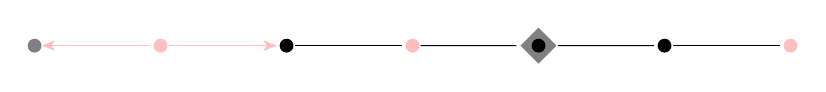
\begin{tikzpicture}[scale=0.8,->,>=stealth',shorten >=1pt,auto,node distance=3cm,
    thick,main node/.style={circle,draw,font=\footnotesize}, small node/.style={circle,font=\footnotesize,inner sep=0pt,minimum size=5pt}]   
   \begin{scope}%[xshift=10cm]
     \node[small node,fill=gray] (b) at (2,5) {};
      \node[small node,fill=pink] (c) at (4,5) {};
      %\node[inner sep=0pt]  (d) at (6,5) {\includegraphics[width=.03\textwidth,right]{robot1.jpg}};
       \node[small node,fill=black] (d) at (6,5) {};
       \node[small node,fill=pink] (e) at (8,5) {};  
       
      \node[diamond, fill=gray]  (f)  at (10,5) {};
      \node[small node,fill=black]   at (10,5) {};
      %\node[small node,fill=pink]  at (10,5) {};
      \node[small node,fill=black] (i) at (12,5) {};
      \node[small node,fill=pink] (j) at (14,5) {};
       \path[<-,line width=0.6pt, color=pink] (b) edge (c);
       \path[->,line width=0.6pt, color=pink] (c) edge (d);
       \path[-,line width=0.3pt]  (d) edge (e);
      \path[-,line width=0.3pt] (e) edge (f);
      \path[-,line width=0.3pt] (f) edge (i);
      \path[-,line width=0.3pt] (i) edge (j);
      %\path[-,line width=0.3pt, color=pink] (f) edge [bend left,-] (8.8,6.8);       

    \end{scope}
  \end{tikzpicture}
\end{frame}

\begin{frame}{Robots: Asynchronous} %%% CYCLE 7 %%%

    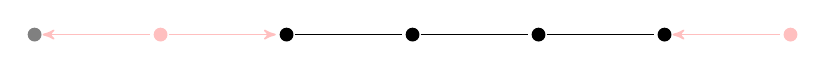
\begin{tikzpicture}[scale=0.8,->,>=stealth',shorten >=1pt,auto,node distance=3cm,
    thick,main node/.style={circle,draw,font=\footnotesize}, small node/.style={circle,font=\footnotesize,inner sep=0pt,minimum size=5pt}]   
   \begin{scope}%[xshift=10cm]
     \node[small node,fill=gray] (b) at (2,5) {};
      \node[small node,fill=pink] (c) at (4,5) {};
      %\node[inner sep=0pt]  (d) at (6,5) {\includegraphics[width=.03\textwidth,right]{robot1.jpg}};
       \node[small node,fill=black] (d) at (6,5) {};
       \node[small node,fill=black] (e) at (8,5) {};    

      \node[small node,fill=black]  (f) at (10,5) {};
      %\node[small node,fill=pink]  at (10,5) {};
      \node[small node,fill=black] (i) at (12,5) {};
      \node[small node,fill=pink] (j) at (14,5) {};
       \path[<-,line width=0.6pt, color=pink] (b) edge (c);
       \path[->,line width=0.6pt, color=pink] (c) edge (d);
       \path[-,line width=0.3pt]  (d) edge (e);
      \path[-,line width=0.3pt] (e) edge (f);
      \path[-,line width=0.3pt] (f) edge (i);
      \path[<-,line width=0.6pt, color=pink] (i) edge (j);
      %\path[-,line width=0.3pt, color=pink] (f) edge [bend left,-] (8.8,6.8);       

    \end{scope}
  \end{tikzpicture}
\end{frame}

\begin{frame}{Robots: Oblivious} %%% CYCLE 7 %%%

    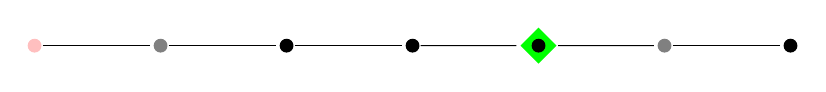
\begin{tikzpicture}[scale=0.8,->,>=stealth',shorten >=1pt,auto,node distance=3cm,
    thick,main node/.style={circle,draw,font=\footnotesize}, small node/.style={circle,font=\footnotesize,inner sep=0pt,minimum size=5pt}]   
   \begin{scope}%[xshift=10cm]
     \node[small node,fill=pink] (b) at (2,5) {};
      \node[small node,fill=gray] (c) at (4,5) {};
      %\node[inner sep=0pt]  (d) at (6,5) {\includegraphics[width=.03\textwidth,right]{robot1.jpg}};
       \node[small node,fill=black] (d) at (6,5) {};
       \node[small node,fill=black] (e) at (8,5) {};    

      \node[diamond, fill=green]  (f) at (10,5) {};
      \node[small node,fill=black]  at (10,5) {};
      \node[small node,fill=gray] (i) at (12,5) {};
      \node[small node,fill=black] (j) at (14,5) {};
       \path[-,line width=0.3pt] (b) edge (c);
       \path[-,line width=0.3pt] (c) edge (d);
       \path[-,line width=0.3pt]  (d) edge (e);
      \path[-,line width=0.3pt] (e) edge (f);
      \path[-,line width=0.3pt] (f) edge (i);
      \path[-,line width=0.3pt] (i) edge (j);
      %\path[-,line width=0.3pt, color=pink] (f) edge [bend left,-] (8.8,6.8);       

    \end{scope}
  \end{tikzpicture}
\end{frame}

%%%%%%%%%%%%%%%%%%%%%%%%%%%%%%%%%%%%%%%%%%%%%%%%%%%%%%
%%%%%%%%%%%%%%%%%%%%%%%%%%%%%%%%%%%%%%%%%%%%%%%%%%%%%%
\miniframeson
\section{\scshape Problem}
\subsection{Exploration}
\begin{frame}{Exploration with termination}
\begin{itemize}
 \item initial configuration with no towers
 \item \textcolor{gray}{all nodes must be visited}
 \item \textcolor{gray}{after finite time robots should stay idle}
\end{itemize}
\end{frame}
\miniframesoff
\begin{frame}{Exploration with termination}
\begin{itemize}
 \item \textcolor{gray}{initial configuration with no towers}
 \item all nodes must be visited
 \item \textcolor{gray}{after finite time robots should stay idle}
\end{itemize}
\end{frame}

\begin{frame}{Exploration with termination}
\begin{itemize}
 \item \textcolor{gray}{initial configuration with no towers}
 \item \textcolor{gray}{all nodes must be visited}
 \item after finite time robots should stay idle
\end{itemize}
\end{frame}
\miniframeson
\subsection{Subproblem 1}
\begin{frame}{Subproblem 1: Setup Phase}

 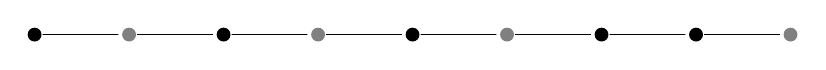
\begin{tikzpicture}[scale=0.6,->,>=stealth',shorten >=1pt,auto,node distance=3cm,
    thick,main node/.style={circle,draw,font=\footnotesize}, small node/.style={circle,font=\footnotesize,inner sep=0pt,minimum size=5pt}]   
   \begin{scope}[yshift=5cm]
     \node[small node,fill=black] (b) at (2,5) {};
      \node[small node,fill=gray] (c) at (4,5) {};
      %\node[inner sep=0pt]  (d) at (6,5) {\includegraphics[width=.03\textwidth,right]{robot1.jpg}};
       \node[small node,fill=black] (d) at (6,5) {};
       \node[small node,fill=gray] (e) at (8,5) {};    
      \node[small node,fill=black]  (f) at (10,5) {};
      %\node[small node,fill=pink]  at (10,5) {};
      \node[small node,fill=gray] (i) at (12,5) {};
      \node[small node,fill=black] (j) at (14,5) {};
      \node[small node,fill=black] (k) at (16,5) {};
      \node[small node,fill=gray] (l) at (18,5) {};
      %\node[small node,fill=gray] (m) at (20,5) {};
       \path[-,line width=0.3pt] (b) edge (c);
       \path[-,line width=0.3pt] (c) edge (d);
       \path[-,line width=0.3pt]  (d) edge (e);
      \path[-,line width=0.3pt] (e) edge (f);
      \path[-,line width=0.3pt] (f) edge (i);
      \path[-,line width=0.3pt] (i) edge (j);
      \path[-,line width=0.3pt] (j) edge (k);
      \path[-,line width=0.3pt] (k) edge (l);
      %\path[-,line width=0.3pt] (l) edge (m);
      %\path[-,line width=0.3pt, color=pink] (f) edge [bend left,-] (8.8,6.8);    
    \end{scope}
  \end{tikzpicture} 
  
  \begin{itemize}
  \item $n$ is odd
  \item  $\# robots$ is odd
 \end{itemize}
 
\end{frame}
\miniframesoff


\begin{frame}{Subproblem 1: Setup Phase}

 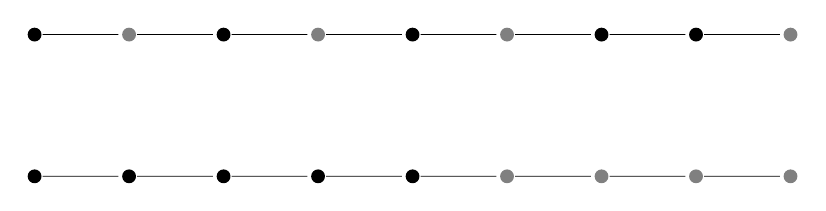
\begin{tikzpicture}[scale=0.6,->,>=stealth',shorten >=1pt,auto,node distance=3cm,
    thick,main node/.style={circle,draw,font=\footnotesize}, small node/.style={circle,font=\footnotesize,inner sep=0pt,minimum size=5pt}]   
   \begin{scope}%[xshift=10cm]
     \node[small node,fill=black] (b) at (2,5) {};
      \node[small node,fill=gray] (c) at (4,5) {};
      %\node[inner sep=0pt]  (d) at (6,5) {\includegraphics[width=.03\textwidth,right]{robot1.jpg}};
       \node[small node,fill=black] (d) at (6,5) {};
       \node[small node,fill=gray] (e) at (8,5) {};    
      \node[small node,fill=black]  (f) at (10,5) {};
      %\node[small node,fill=pink]  at (10,5) {};
      \node[small node,fill=gray] (i) at (12,5) {};
      \node[small node,fill=black] (j) at (14,5) {};
      \node[small node,fill=black] (k) at (16,5) {};
      \node[small node,fill=gray] (l) at (18,5) {};
      %\node[small node,fill=gray] (m) at (20,5) {};
       \path[-,line width=0.3pt] (b) edge (c);
       \path[-,line width=0.3pt] (c) edge (d);
       \path[-,line width=0.3pt]  (d) edge (e);
      \path[-,line width=0.3pt] (e) edge (f);
      \path[-,line width=0.3pt] (f) edge (i);
      \path[-,line width=0.3pt] (i) edge (j);
      \path[-,line width=0.3pt] (j) edge (k);
      \path[-,line width=0.3pt] (k) edge (l);
      %\path[-,line width=0.3pt] (l) edge (m);
      %\path[-,line width=0.3pt, color=pink] (f) edge [bend left,-] (8.8,6.8);    
    \end{scope}
     \begin{scope}[yshift=-3cm]
     \node[small node,fill=black] (b) at (2,5) {};
      \node[small node,fill=black] (c) at (4,5) {};
      %\node[inner sep=0pt]  (d) at (6,5) {\includegraphics[width=.03\textwidth,right]{robot1.jpg}};
       \node[small node,fill=black] (d) at (6,5) {};
       \node[small node,fill=black] (e) at (8,5) {};    
      \node[small node,fill=black]  (f) at (10,5) {};
      %\node[small node,fill=pink]  at (10,5) {};
      \node[small node,fill=gray] (i) at (12,5) {};
      \node[small node,fill=gray] (j) at (14,5) {};
      \node[small node,fill=gray] (k) at (16,5) {};
      \node[small node,fill=gray] (l) at (18,5) {};
      %\node[small node,fill=gray] (m) at (20,5) {};
       \path[-,line width=0.3pt] (b) edge (c);
       \path[-,line width=0.3pt] (c) edge (d);
       \path[-,line width=0.3pt]  (d) edge (e);
      \path[-,line width=0.3pt] (e) edge (f);
      \path[-,line width=0.3pt] (f) edge (i);
      \path[-,line width=0.3pt] (i) edge (j);
      \path[-,line width=0.3pt] (j) edge (k);
      \path[-,line width=0.3pt] (k) edge (l);
      %\path[-,line width=0.3pt] (l) edge (m);
      %\path[-,line width=0.3pt, color=pink] (f) edge [bend left,-] (8.8,6.8);       

    \end{scope}
  \end{tikzpicture} 
\end{frame}

\begin{frame}{Subproblem 1: Setup Phase}



 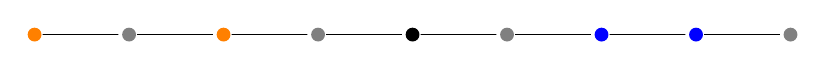
\begin{tikzpicture}[scale=0.6,->,>=stealth',shorten >=1pt,auto,node distance=3cm,
    thick,main node/.style={circle,draw,font=\footnotesize}, small node/.style={circle,font=\footnotesize,inner sep=0pt,minimum size=5pt}]   
   \begin{scope}%[xshift=10cm]
     \node[small node,fill=orange] (b) at (2,5) {};
      \node[small node,fill=gray] (c) at (4,5) {};
      %\node[inner sep=0pt]  (d) at (6,5) {\includegraphics[width=.03\textwidth,right]{robot1.jpg}};
      \node[small node,fill=orange] (d) at (6,5) {};
      \node[small node,fill=gray] (e) at (8,5) {};    
      \node[small node,fill=black]  (f) at (10,5) {};
      %\node[small node,fill=pink]  at (10,5) {};
      \node[small node,fill=gray] (i) at (12,5) {};
      \node[small node,fill=blue] (j) at (14,5) {};
      \node[small node,fill=blue] (k) at (16,5) {};
      \node[small node,fill=gray] (l) at (18,5) {};
      %\node[small node,fill=gray] (m) at (20,5) {};
       \path[-,line width=0.3pt] (b) edge (c);
       \path[-,line width=0.3pt] (c) edge (d);
       \path[-,line width=0.3pt]  (d) edge (e);
      \path[-,line width=0.3pt] (e) edge (f);
      \path[-,line width=0.3pt] (f) edge (i);
      \path[-,line width=0.3pt] (i) edge (j);
      \path[-,line width=0.3pt] (j) edge (k);
      \path[-,line width=0.3pt] (k) edge (l);
      %\path[-,line width=0.3pt] (l) edge (m);
      %\path[-,line width=0.3pt, color=pink] (f) edge [bend left,-] (8.8,6.8);       

    \end{scope}
  \end{tikzpicture} \\ \vspace{1cm}


\textcolor{orange}{ $h_{1}$ } = \# robots in $[v_{1}...v_{\lfloor n/2\rfloor}]$ \\ \vspace{1cm}
\textcolor{blue}{ $h_{2}$ } = \# robots in $[v_{\lceil n/2\rceil...v_{n}}]$ \\ \vspace{1cm}
  


\end{frame}


\begin{frame}{Subproblem 1: Setup Phase}


 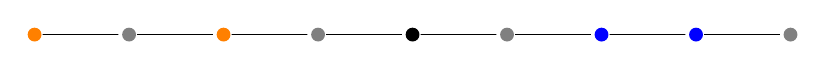
\begin{tikzpicture}[scale=0.6,->,>=stealth',shorten >=1pt,auto,node distance=3cm,
    thick,main node/.style={circle,draw,font=\footnotesize}, small node/.style={circle,font=\footnotesize,inner sep=0pt,minimum size=5pt}]   
   \begin{scope}%[xshift=10cm]
     \node[small node,fill=orange] (b) at (2,5) {};
      \node[small node,fill=gray] (c) at (4,5) {};
      %\node[inner sep=0pt]  (d) at (6,5) {\includegraphics[width=.03\textwidth,right]{robot1.jpg}};
      \node[small node,fill=orange] (d) at (6,5) {};
      \node[small node,fill=gray] (e) at (8,5) {};    
      \node[small node,fill=black]  (f) at (10,5) {};
      %\node[small node,fill=pink]  at (10,5) {};
      \node[small node,fill=gray] (i) at (12,5) {};
      \node[small node,fill=blue] (j) at (14,5) {};
      \node[small node,fill=blue] (k) at (16,5) {};
      \node[small node,fill=gray] (l) at (18,5) {};
      %\node[small node,fill=gray] (m) at (20,5) {};
       \path[-,line width=0.3pt] (b) edge (c);
       \path[-,line width=0.3pt] (c) edge (d);
       \path[-,line width=0.3pt]  (d) edge (e);
      \path[-,line width=0.3pt] (e) edge (f);
      \path[-,line width=0.3pt] (f) edge (i);
      \path[-,line width=0.3pt] (i) edge (j);
      \path[-,line width=0.3pt] (j) edge (k);
      \path[-,line width=0.3pt] (k) edge (l);
      %\path[-,line width=0.3pt] (l) edge (m);
      %\path[-,line width=0.3pt, color=pink] (f) edge [bend left,-] (8.8,6.8);       

    \end{scope}
  \end{tikzpicture} \\


\begin{itemize}
 \item $h_{1} = h_{2}$ \hfill \\
 \begin{itemize}
  \item $player = v_{n/2}$
  \item  $destination = any neighbor$
 \end{itemize}
 \item $h_{1} \neq h_{2}$ \hfill \\
\end{itemize}

\end{frame}

\begin{frame}{Subproblem 1: Setup Phase}


 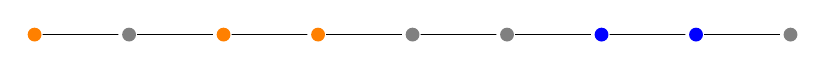
\begin{tikzpicture}[scale=0.6,->,>=stealth',shorten >=1pt,auto,node distance=3cm,
    thick,main node/.style={circle,draw,font=\footnotesize}, small node/.style={circle,font=\footnotesize,inner sep=0pt,minimum size=5pt}]   
   \begin{scope}%[xshift=10cm]
     \node[small node,fill=orange] (b) at (2,5) {};
      \node[small node,fill=gray] (c) at (4,5) {};
      %\node[inner sep=0pt]  (d) at (6,5) {\includegraphics[width=.03\textwidth,right]{robot1.jpg}};
      \node[small node,fill=orange] (d) at (6,5) {};
      \node[small node,fill=orange] (e) at (8,5) {};    
      \node[small node,fill=gray]  (f) at (10,5) {};
      %\node[small node,fill=pink]  at (10,5) {};
      \node[small node,fill=gray] (i) at (12,5) {};
      \node[small node,fill=blue] (j) at (14,5) {};
      \node[small node,fill=blue] (k) at (16,5) {};
      \node[small node,fill=gray] (l) at (18,5) {};
      %\node[small node,fill=gray] (m) at (20,5) {};
       \path[-,line width=0.3pt] (b) edge (c);
       \path[-,line width=0.3pt] (c) edge (d);
       \path[-,line width=0.3pt]  (d) edge (e);
      \path[-,line width=0.3pt] (e) edge (f);
      \path[-,line width=0.3pt] (f) edge (i);
      \path[-,line width=0.3pt] (i) edge (j);
      \path[-,line width=0.3pt] (j) edge (k);
      \path[-,line width=0.3pt] (k) edge (l);
      %\path[-,line width=0.3pt] (l) edge (m);
      %\path[-,line width=0.3pt, color=pink] (f) edge [bend left,-] (8.8,6.8);       

    \end{scope}
  \end{tikzpicture} \\


\begin{itemize}
 \item $h_{1} = h_{2}$ \hfill \\
 \item $h_{1} \neq h_{2}$ \hfill \\
 \begin{itemize}
  \item $left - right$ direction from $min{h_{1}, h_{2}} to max{h_{1}, h_{2}}$
  \item  If my right neighbor $y$ is empty \\ 
  \- \- \- \- \- \- I am a $player$ and $y$ is my $destination$

 \end{itemize}

 %\item if $h_{1} = h_{2}$
 %\item \textcolor{gray}{all nodes must be visited}
 %\item \textcolor{gray}{after finite time robots should stay idle}
\end{itemize}

\end{frame}

%%%%%%%%%%%%%%     SETUP PHASE %%%%%%%%%%%%%%%%%%%%%
\begin{frame}{Subproblem 1: Setup Phase}
 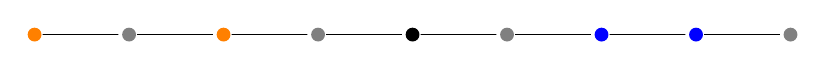
\begin{tikzpicture}[scale=0.6,->,>=stealth',shorten >=1pt,auto,node distance=3cm,
    thick,main node/.style={circle,draw,font=\footnotesize}, small node/.style={circle,font=\footnotesize,inner sep=0pt,minimum size=5pt}]   
   \begin{scope}%[xshift=10cm]
     \node[small node,fill=orange] (b) at (2,5) {};
      \node[small node,fill=gray] (c) at (4,5) {};
      %\node[inner sep=0pt]  (d) at (6,5) {\includegraphics[width=.03\textwidth,right]{robot1.jpg}};
      \node[small node,fill=orange] (d) at (6,5) {};
      \node[small node,fill=gray] (e) at (8,5) {};    
      \node[small node,fill=black]  (f) at (10,5) {};
      %\node[small node,fill=pink]  at (10,5) {};
      \node[small node,fill=gray] (i) at (12,5) {};
      \node[small node,fill=blue] (j) at (14,5) {};
      \node[small node,fill=blue] (k) at (16,5) {};
      \node[small node,fill=gray] (l) at (18,5) {};
      %\node[small node,fill=gray] (m) at (20,5) {};
       \path[-,line width=0.3pt] (b) edge (c);
       \path[-,line width=0.3pt] (c) edge (d);
       \path[-,line width=0.3pt]  (d) edge (e);
      \path[-,line width=0.3pt] (e) edge (f);
      \path[-,line width=0.3pt] (f) edge (i);
      \path[-,line width=0.3pt] (i) edge (j);
      \path[-,line width=0.3pt] (j) edge (k);
      \path[-,line width=0.3pt] (k) edge (l);
      %\path[-,line width=0.3pt] (l) edge (m);
      %\path[-,line width=0.3pt, color=pink] (f) edge [bend left,-] (8.8,6.8);       
    \end{scope}
  \end{tikzpicture} \\
\end{frame}
\begin{frame}{Subproblem 1: Setup Phase}
 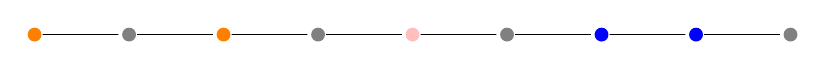
\begin{tikzpicture}[scale=0.6,->,>=stealth',shorten >=1pt,auto,node distance=3cm,
    thick,main node/.style={circle,draw,font=\footnotesize}, small node/.style={circle,font=\footnotesize,inner sep=0pt,minimum size=5pt}]   
   \begin{scope}%[xshift=10cm]
     \node[small node,fill=orange] (b) at (2,5) {};
      \node[small node,fill=gray] (c) at (4,5) {};
      %\node[inner sep=0pt]  (d) at (6,5) {\includegraphics[width=.03\textwidth,right]{robot1.jpg}};
      \node[small node,fill=orange] (d) at (6,5) {};
      \node[small node,fill=gray] (e) at (8,5) {};    
      \node[small node,fill=pink]  (f) at (10,5) {};
      %\node[small node,fill=pink]  at (10,5) {};
      \node[small node,fill=gray] (i) at (12,5) {};
      \node[small node,fill=blue] (j) at (14,5) {};
      \node[small node,fill=blue] (k) at (16,5) {};
      \node[small node,fill=gray] (l) at (18,5) {};
      %\node[small node,fill=gray] (m) at (20,5) {};
       \path[-,line width=0.3pt] (b) edge (c);
       \path[-,line width=0.3pt] (c) edge (d);
       \path[-,line width=0.3pt]  (d) edge (e);
      \path[-,line width=0.3pt] (e) edge (f);
      \path[-,line width=0.3pt] (f) edge (i);
      \path[-,line width=0.3pt] (i) edge (j);
      \path[-,line width=0.3pt] (j) edge (k);
      \path[-,line width=0.3pt] (k) edge (l);
      %\path[-,line width=0.3pt] (l) edge (m);
      %\path[-,line width=0.3pt, color=pink] (f) edge [bend left,-] (8.8,6.8);       
    \end{scope}
  \end{tikzpicture} \\
\end{frame}
\begin{frame}{Subproblem 1: Setup Phase}
 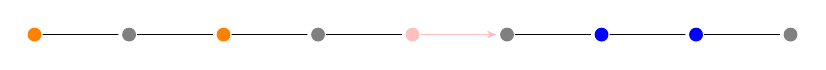
\begin{tikzpicture}[scale=0.6,->,>=stealth',shorten >=1pt,auto,node distance=3cm,
    thick,main node/.style={circle,draw,font=\footnotesize}, small node/.style={circle,font=\footnotesize,inner sep=0pt,minimum size=5pt}]   
   \begin{scope}%[xshift=10cm]
     \node[small node,fill=orange] (b) at (2,5) {};
      \node[small node,fill=gray] (c) at (4,5) {};
      %\node[inner sep=0pt]  (d) at (6,5) {\includegraphics[width=.03\textwidth,right]{robot1.jpg}};
      \node[small node,fill=orange] (d) at (6,5) {};
      \node[small node,fill=gray] (e) at (8,5) {};    
      \node[small node,fill=pink]  (f) at (10,5) {};
      %\node[small node,fill=pink]  at (10,5) {};
      \node[small node,fill=gray] (i) at (12,5) {};
      \node[small node,fill=blue] (j) at (14,5) {};
      \node[small node,fill=blue] (k) at (16,5) {};
      \node[small node,fill=gray] (l) at (18,5) {};
      %\node[small node,fill=gray] (m) at (20,5) {};
       \path[-,line width=0.3pt] (b) edge (c);
       \path[-,line width=0.3pt] (c) edge (d);
       \path[-,line width=0.3pt]  (d) edge (e);
      \path[-,line width=0.3pt] (e) edge (f);
      \path[->,line width=0.3pt, color=pink] (f) edge (i);
      \path[-,line width=0.3pt] (i) edge (j);
      \path[-,line width=0.3pt] (j) edge (k);
      \path[-,line width=0.3pt] (k) edge (l);
      %\path[-,line width=0.3pt] (l) edge (m);
      %\path[-,line width=0.3pt, color=pink] (f) edge [bend left,-] (8.8,6.8);       
    \end{scope}
  \end{tikzpicture} \\
\end{frame}
\begin{frame}{Subproblem 1: Setup Phase}
 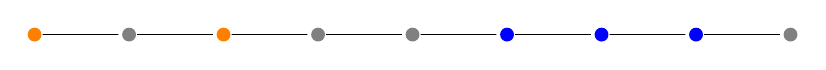
\begin{tikzpicture}[scale=0.6,->,>=stealth',shorten >=1pt,auto,node distance=3cm,
    thick,main node/.style={circle,draw,font=\footnotesize}, small node/.style={circle,font=\footnotesize,inner sep=0pt,minimum size=5pt}]   
   \begin{scope}%[xshift=10cm]
     \node[small node,fill=orange] (b) at (2,5) {};
      \node[small node,fill=gray] (c) at (4,5) {};
      %\node[inner sep=0pt]  (d) at (6,5) {\includegraphics[width=.03\textwidth,right]{robot1.jpg}};
      \node[small node,fill=orange] (d) at (6,5) {};
      \node[small node,fill=gray] (e) at (8,5) {};    
      \node[small node,fill=gray]  (f) at (10,5) {};
      %\node[small node,fill=pink]  at (10,5) {};
      \node[small node,fill=blue] (i) at (12,5) {};
      \node[small node,fill=blue] (j) at (14,5) {};
      \node[small node,fill=blue] (k) at (16,5) {};
      \node[small node,fill=gray] (l) at (18,5) {};
      %\node[small node,fill=gray] (m) at (20,5) {};
       \path[-,line width=0.3pt] (b) edge (c);
       \path[-,line width=0.3pt] (c) edge (d);
       \path[-,line width=0.3pt]  (d) edge (e);
      \path[-,line width=0.3pt] (e) edge (f);
      \path[-,line width=0.3pt] (f) edge (i);
      \path[-,line width=0.3pt] (i) edge (j);
      \path[-,line width=0.3pt] (j) edge (k);
      \path[-,line width=0.3pt] (k) edge (l);
      %\path[-,line width=0.3pt] (l) edge (m);
      %\path[-,line width=0.3pt, color=pink] (f) edge [bend left,-] (8.8,6.8);       
    \end{scope}
  \end{tikzpicture} \\
\end{frame}
\begin{frame}{Subproblem 1: Setup Phase}
 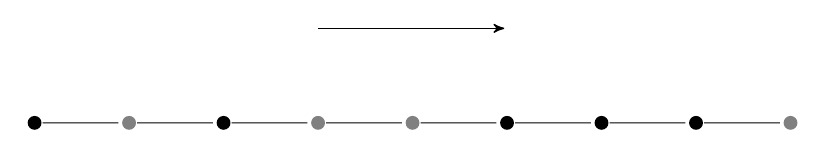
\begin{tikzpicture}[scale=0.6,->,>=stealth',shorten >=1pt,auto,node distance=3cm,
    thick,main node/.style={circle,draw,font=\footnotesize}, small node/.style={circle,font=\footnotesize,inner sep=0pt,minimum size=5pt}]   
   \begin{scope}%[xshift=10cm]
     \node[small node,fill=black] (b) at (2,5) {};
      \node[small node,fill=gray] (c) at (4,5) {};
      %\node[inner sep=0pt]  (d) at (6,5) {\includegraphics[width=.03\textwidth,right]{robot1.jpg}};
      \node[small node,fill=black] (d) at (6,5) {};
      \node[small node,fill=gray] (e) at (8,5) {};    
      \node[small node,fill=gray]  (f) at (10,5) {};
      %\node[small node,fill=pink]  at (10,5) {};
      \node[small node,fill=black] (i) at (12,5) {};
      \node[small node,fill=black] (j) at (14,5) {};
      \node[small node,fill=black] (k) at (16,5) {};
      \node[small node,fill=gray] (l) at (18,5) {};
      %\node[small node,fill=gray] (m) at (20,5) {};
       \path[-,line width=0.3pt] (b) edge (c);
       \path[-,line width=0.3pt] (c) edge (d);
       \path[-,line width=0.3pt]  (d) edge (e);
      \path[-,line width=0.3pt] (e) edge (f);
      \path[-,line width=0.3pt] (f) edge (i);
      \path[-,line width=0.3pt] (i) edge (j);
      \path[-,line width=0.3pt] (j) edge (k);
      \path[-,line width=0.3pt] (k) edge (l);
      \path[->, line width=0.5pt] (8,7) edge (12,7);
      %\path[-,line width=0.3pt] (l) edge (m);
      %\path[-,line width=0.3pt, color=pink] (f) edge [bend left,-] (8.8,6.8);       
    \end{scope}
  \end{tikzpicture} \\
\end{frame}
\begin{frame}{Subproblem 1: Setup Phase}
 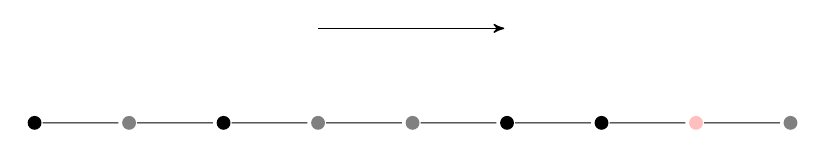
\begin{tikzpicture}[scale=0.6,->,>=stealth',shorten >=1pt,auto,node distance=3cm,
    thick,main node/.style={circle,draw,font=\footnotesize}, small node/.style={circle,font=\footnotesize,inner sep=0pt,minimum size=5pt}]   
   \begin{scope}%[xshift=10cm]
     \node[small node,fill=black] (b) at (2,5) {};
      \node[small node,fill=gray] (c) at (4,5) {};
      %\node[inner sep=0pt]  (d) at (6,5) {\includegraphics[width=.03\textwidth,right]{robot1.jpg}};
      \node[small node,fill=black] (d) at (6,5) {};
      \node[small node,fill=gray] (e) at (8,5) {};    
      \node[small node,fill=gray]  (f) at (10,5) {};
      %\node[small node,fill=pink]  at (10,5) {};
      \node[small node,fill=black] (i) at (12,5) {};
      \node[small node,fill=black] (j) at (14,5) {};
      \node[small node,fill=pink] (k) at (16,5) {};
      \node[small node,fill=gray] (l) at (18,5) {};
      %\node[small node,fill=gray] (m) at (20,5) {};
       \path[-,line width=0.3pt] (b) edge (c);
       \path[-,line width=0.3pt] (c) edge (d);
       \path[-,line width=0.3pt]  (d) edge (e);
      \path[-,line width=0.3pt] (e) edge (f);
      \path[-,line width=0.3pt] (f) edge (i);
      \path[-,line width=0.3pt] (i) edge (j);
      \path[-,line width=0.3pt] (j) edge (k);
      \path[-,line width=0.3pt] (k) edge (l);
      \path[->, line width=0.5pt] (8,7) edge (12,7);
      %\path[-,line width=0.3pt] (l) edge (m);
      %\path[-,line width=0.3pt, color=pink] (f) edge [bend left,-] (8.8,6.8);       
    \end{scope}
  \end{tikzpicture} \\
\end{frame}
\begin{frame}{Subproblem 1: Setup Phase}
 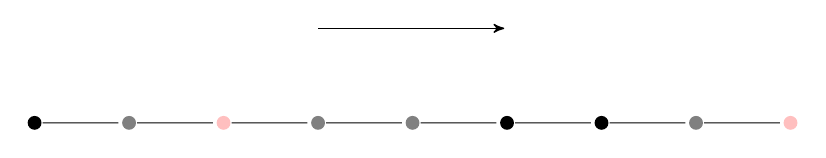
\begin{tikzpicture}[scale=0.6,->,>=stealth',shorten >=1pt,auto,node distance=3cm,
    thick,main node/.style={circle,draw,font=\footnotesize}, small node/.style={circle,font=\footnotesize,inner sep=0pt,minimum size=5pt}]   
   \begin{scope}%[xshift=10cm]
     \node[small node,fill=black] (b) at (2,5) {};
      \node[small node,fill=gray] (c) at (4,5) {};
      %\node[inner sep=0pt]  (d) at (6,5) {\includegraphics[width=.03\textwidth,right]{robot1.jpg}};
      \node[small node,fill=pink] (d) at (6,5) {};
      \node[small node,fill=gray] (e) at (8,5) {};    
      \node[small node,fill=gray]  (f) at (10,5) {};
      %\node[small node,fill=pink]  at (10,5) {};
      \node[small node,fill=black] (i) at (12,5) {};
      \node[small node,fill=black] (j) at (14,5) {};
      \node[small node,fill=gray] (k) at (16,5) {};
      \node[small node,fill=pink] (l) at (18,5) {};
      %\node[small node,fill=gray] (m) at (20,5) {};
       \path[-,line width=0.3pt] (b) edge (c);
       \path[-,line width=0.3pt] (c) edge (d);
       \path[-,line width=0.3pt]  (d) edge (e);
      \path[-,line width=0.3pt] (e) edge (f);
      \path[-,line width=0.3pt] (f) edge (i);
      \path[-,line width=0.3pt] (i) edge (j);
      \path[-,line width=0.3pt] (j) edge (k);
      \path[-,line width=0.3pt] (k) edge (l);
      \path[->, line width=0.5pt] (8,7) edge (12,7);
      %\path[-,line width=0.3pt] (l) edge (m);
      %\path[-,line width=0.3pt, color=pink] (f) edge [bend left,-] (8.8,6.8);       
    \end{scope}
  \end{tikzpicture} \\
\end{frame}
\begin{frame}{Subproblem 1: Setup Phase}
 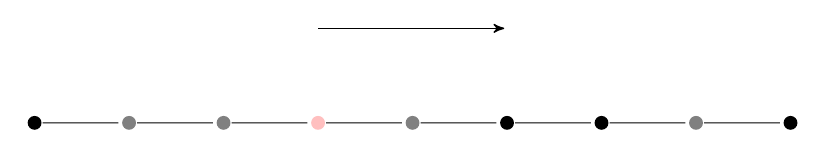
\begin{tikzpicture}[scale=0.6,->,>=stealth',shorten >=1pt,auto,node distance=3cm,
    thick,main node/.style={circle,draw,font=\footnotesize}, small node/.style={circle,font=\footnotesize,inner sep=0pt,minimum size=5pt}]   
   \begin{scope}%[xshift=10cm]
     \node[small node,fill=black] (b) at (2,5) {};
      \node[small node,fill=gray] (c) at (4,5) {};
      %\node[inner sep=0pt]  (d) at (6,5) {\includegraphics[width=.03\textwidth,right]{robot1.jpg}};
      \node[small node,fill=gray] (d) at (6,5) {};
      \node[small node,fill=pink] (e) at (8,5) {};    
      \node[small node,fill=gray]  (f) at (10,5) {};
      %\node[small node,fill=pink]  at (10,5) {};
      \node[small node,fill=black] (i) at (12,5) {};
      \node[small node,fill=black] (j) at (14,5) {};
      \node[small node,fill=gray] (k) at (16,5) {};
      \node[small node,fill=black] (l) at (18,5) {};
      %\node[small node,fill=gray] (m) at (20,5) {};
       \path[-,line width=0.3pt] (b) edge (c);
       \path[-,line width=0.3pt] (c) edge (d);
       \path[-,line width=0.3pt]  (d) edge (e);
      \path[-,line width=0.3pt] (e) edge (f);
      \path[-,line width=0.3pt] (f) edge (i);
      \path[-,line width=0.3pt] (i) edge (j);
      \path[-,line width=0.3pt] (j) edge (k);
      \path[-,line width=0.3pt] (k) edge (l);
      \path[->, line width=0.5pt] (8,7) edge (12,7);
      %\path[-,line width=0.3pt] (l) edge (m);
      %\path[-,line width=0.3pt, color=pink] (f) edge [bend left,-] (8.8,6.8);       
    \end{scope}
  \end{tikzpicture} \\
\end{frame}
\begin{frame}{Subproblem 1: Setup Phase}
 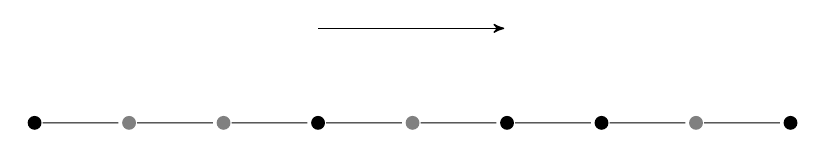
\begin{tikzpicture}[scale=0.6,->,>=stealth',shorten >=1pt,auto,node distance=3cm,
    thick,main node/.style={circle,draw,font=\footnotesize}, small node/.style={circle,font=\footnotesize,inner sep=0pt,minimum size=5pt}]   
   \begin{scope}%[xshift=10cm]
     \node[small node,fill=black] (b) at (2,5) {};
      \node[small node,fill=gray] (c) at (4,5) {};
      %\node[inner sep=0pt]  (d) at (6,5) {\includegraphics[width=.03\textwidth,right]{robot1.jpg}};
      \node[small node,fill=gray] (d) at (6,5) {};
      \node[small node,fill=black] (e) at (8,5) {};    
      \node[small node,fill=gray]  (f) at (10,5) {};
      %\node[small node,fill=pink]  at (10,5) {};
      \node[small node,fill=black] (i) at (12,5) {};
      \node[small node,fill=black] (j) at (14,5) {};
      \node[small node,fill=gray] (k) at (16,5) {};
      \node[small node,fill=black] (l) at (18,5) {};
      %\node[small node,fill=gray] (m) at (20,5) {};
       \path[-,line width=0.3pt] (b) edge (c);
       \path[-,line width=0.3pt] (c) edge (d);
       \path[-,line width=0.3pt]  (d) edge (e);
      \path[-,line width=0.3pt] (e) edge (f);
      \path[-,line width=0.3pt] (f) edge (i);
      \path[-,line width=0.3pt] (i) edge (j);
      \path[-,line width=0.3pt] (j) edge (k);
      \path[-,line width=0.3pt] (k) edge (l);
      \path[->, line width=0.5pt] (8,7) edge (12,7);
      %\path[-,line width=0.3pt] (l) edge (m);
      %\path[-,line width=0.3pt, color=pink] (f) edge [bend left,-] (8.8,6.8);       
    \end{scope}
  \end{tikzpicture} \\
\end{frame}
\begin{frame}{Subproblem 1: Setup Phase}
 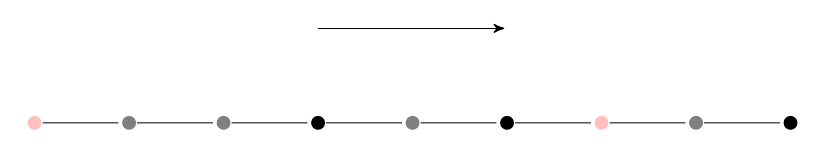
\begin{tikzpicture}[scale=0.6,->,>=stealth',shorten >=1pt,auto,node distance=3cm,
    thick,main node/.style={circle,draw,font=\footnotesize}, small node/.style={circle,font=\footnotesize,inner sep=0pt,minimum size=5pt}]   
   \begin{scope}%[xshift=10cm]
     \node[small node,fill=pink] (b) at (2,5) {};
      \node[small node,fill=gray] (c) at (4,5) {};
      %\node[inner sep=0pt]  (d) at (6,5) {\includegraphics[width=.03\textwidth,right]{robot1.jpg}};
      \node[small node,fill=gray] (d) at (6,5) {};
      \node[small node,fill=black] (e) at (8,5) {};    
      \node[small node,fill=gray]  (f) at (10,5) {};
      %\node[small node,fill=pink]  at (10,5) {};
      \node[small node,fill=black] (i) at (12,5) {};
      \node[small node,fill=pink] (j) at (14,5) {};
      \node[small node,fill=gray] (k) at (16,5) {};
      \node[small node,fill=black] (l) at (18,5) {};
      %\node[small node,fill=gray] (m) at (20,5) {};
       \path[-,line width=0.3pt] (b) edge (c);
       \path[-,line width=0.3pt] (c) edge (d);
       \path[-,line width=0.3pt]  (d) edge (e);
      \path[-,line width=0.3pt] (e) edge (f);
      \path[-,line width=0.3pt] (f) edge (i);
      \path[-,line width=0.3pt] (i) edge (j);
      \path[-,line width=0.3pt] (j) edge (k);
      \path[-,line width=0.3pt] (k) edge (l);
      \path[->, line width=0.5pt] (8,7) edge (12,7);
      %\path[-,line width=0.3pt] (l) edge (m);
      %\path[-,line width=0.3pt, color=pink] (f) edge [bend left,-] (8.8,6.8);       
    \end{scope}
  \end{tikzpicture} \\
\end{frame}
\begin{frame}{Subproblem 1: Setup Phase}
 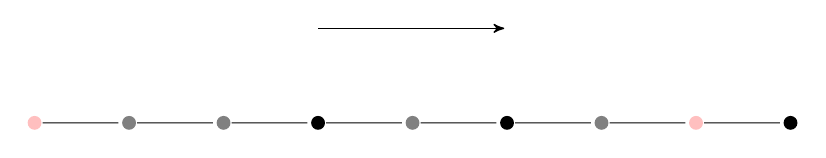
\begin{tikzpicture}[scale=0.6,->,>=stealth',shorten >=1pt,auto,node distance=3cm,
    thick,main node/.style={circle,draw,font=\footnotesize}, small node/.style={circle,font=\footnotesize,inner sep=0pt,minimum size=5pt}]   
   \begin{scope}%[xshift=10cm]
     \node[small node,fill=pink] (b) at (2,5) {};
      \node[small node,fill=gray] (c) at (4,5) {};
      %\node[inner sep=0pt]  (d) at (6,5) {\includegraphics[width=.03\textwidth,right]{robot1.jpg}};
      \node[small node,fill=gray] (d) at (6,5) {};
      \node[small node,fill=black] (e) at (8,5) {};    
      \node[small node,fill=gray]  (f) at (10,5) {};
      %\node[small node,fill=pink]  at (10,5) {};
      \node[small node,fill=black] (i) at (12,5) {};
      \node[small node,fill=gray] (j) at (14,5) {};
      \node[small node,fill=pink] (k) at (16,5) {};
      \node[small node,fill=black] (l) at (18,5) {};
      %\node[small node,fill=gray] (m) at (20,5) {};
       \path[-,line width=0.3pt] (b) edge (c);
       \path[-,line width=0.3pt] (c) edge (d);
       \path[-,line width=0.3pt]  (d) edge (e);
      \path[-,line width=0.3pt] (e) edge (f);
      \path[-,line width=0.3pt] (f) edge (i);
      \path[-,line width=0.3pt] (i) edge (j);
      \path[-,line width=0.3pt] (j) edge (k);
      \path[-,line width=0.3pt] (k) edge (l);
      \path[->, line width=0.5pt] (8,7) edge (12,7);
      %\path[-,line width=0.3pt] (l) edge (m);
      %\path[-,line width=0.3pt, color=pink] (f) edge [bend left,-] (8.8,6.8);       
    \end{scope}
  \end{tikzpicture} \\
\end{frame}
\begin{frame}{Subproblem 1: Setup Phase}
 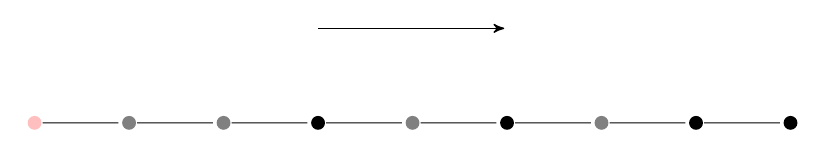
\begin{tikzpicture}[scale=0.6,->,>=stealth',shorten >=1pt,auto,node distance=3cm,
    thick,main node/.style={circle,draw,font=\footnotesize}, small node/.style={circle,font=\footnotesize,inner sep=0pt,minimum size=5pt}]   
   \begin{scope}%[xshift=10cm]
     \node[small node,fill=pink] (b) at (2,5) {};
      \node[small node,fill=gray] (c) at (4,5) {};
      %\node[inner sep=0pt]  (d) at (6,5) {\includegraphics[width=.03\textwidth,right]{robot1.jpg}};
      \node[small node,fill=gray] (d) at (6,5) {};
      \node[small node,fill=black] (e) at (8,5) {};    
      \node[small node,fill=gray]  (f) at (10,5) {};
      %\node[small node,fill=pink]  at (10,5) {};
      \node[small node,fill=black] (i) at (12,5) {};
      \node[small node,fill=gray] (j) at (14,5) {};
      \node[small node,fill=black] (k) at (16,5) {};
      \node[small node,fill=black] (l) at (18,5) {};
      %\node[small node,fill=gray] (m) at (20,5) {};
       \path[-,line width=0.3pt] (b) edge (c);
       \path[-,line width=0.3pt] (c) edge (d);
       \path[-,line width=0.3pt]  (d) edge (e);
      \path[-,line width=0.3pt] (e) edge (f);
      \path[-,line width=0.3pt] (f) edge (i);
      \path[-,line width=0.3pt] (i) edge (j);
      \path[-,line width=0.3pt] (j) edge (k);
      \path[-,line width=0.3pt] (k) edge (l);
      \path[->, line width=0.5pt] (8,7) edge (12,7);
      %\path[-,line width=0.3pt] (l) edge (m);
      %\path[-,line width=0.3pt, color=pink] (f) edge [bend left,-] (8.8,6.8);       
    \end{scope}
  \end{tikzpicture} \\
\end{frame}
\begin{frame}{Subproblem 1: Setup Phase}
 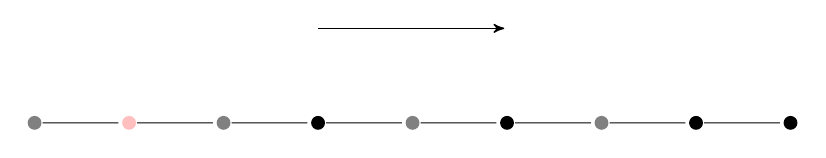
\begin{tikzpicture}[scale=0.6,->,>=stealth',shorten >=1pt,auto,node distance=3cm,
    thick,main node/.style={circle,draw,font=\footnotesize}, small node/.style={circle,font=\footnotesize,inner sep=0pt,minimum size=5pt}]   
   \begin{scope}%[xshift=10cm]
     \node[small node,fill=gray] (b) at (2,5) {};
      \node[small node,fill=pink] (c) at (4,5) {};
      %\node[inner sep=0pt]  (d) at (6,5) {\includegraphics[width=.03\textwidth,right]{robot1.jpg}};
      \node[small node,fill=gray] (d) at (6,5) {};
      \node[small node,fill=black] (e) at (8,5) {};    
      \node[small node,fill=gray]  (f) at (10,5) {};
      %\node[small node,fill=pink]  at (10,5) {};
      \node[small node,fill=black] (i) at (12,5) {};
      \node[small node,fill=gray] (j) at (14,5) {};
      \node[small node,fill=black] (k) at (16,5) {};
      \node[small node,fill=black] (l) at (18,5) {};
      %\node[small node,fill=gray] (m) at (20,5) {};
       \path[-,line width=0.3pt] (b) edge (c);
       \path[-,line width=0.3pt] (c) edge (d);
       \path[-,line width=0.3pt]  (d) edge (e);
      \path[-,line width=0.3pt] (e) edge (f);
      \path[-,line width=0.3pt] (f) edge (i);
      \path[-,line width=0.3pt] (i) edge (j);
      \path[-,line width=0.3pt] (j) edge (k);
      \path[-,line width=0.3pt] (k) edge (l);
      \path[->, line width=0.5pt] (8,7) edge (12,7);
      %\path[-,line width=0.3pt] (l) edge (m);
      %\path[-,line width=0.3pt, color=pink] (f) edge [bend left,-] (8.8,6.8);       
    \end{scope}
  \end{tikzpicture} \\
\end{frame}
\begin{frame}{Subproblem 1: Setup Phase}
 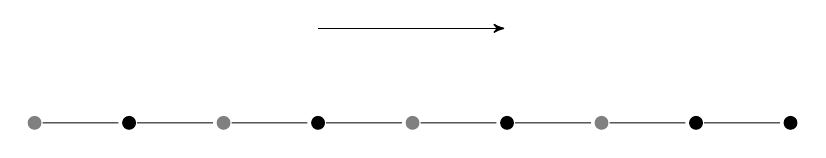
\begin{tikzpicture}[scale=0.6,->,>=stealth',shorten >=1pt,auto,node distance=3cm,
    thick,main node/.style={circle,draw,font=\footnotesize}, small node/.style={circle,font=\footnotesize,inner sep=0pt,minimum size=5pt}]   
   \begin{scope}%[xshift=10cm]
     \node[small node,fill=gray] (b) at (2,5) {};
      \node[small node,fill=black] (c) at (4,5) {};
      %\node[inner sep=0pt]  (d) at (6,5) {\includegraphics[width=.03\textwidth,right]{robot1.jpg}};
      \node[small node,fill=gray] (d) at (6,5) {};
      \node[small node,fill=black] (e) at (8,5) {};    
      \node[small node,fill=gray]  (f) at (10,5) {};
      %\node[small node,fill=pink]  at (10,5) {};
      \node[small node,fill=black] (i) at (12,5) {};
      \node[small node,fill=gray] (j) at (14,5) {};
      \node[small node,fill=black] (k) at (16,5) {};
      \node[small node,fill=black] (l) at (18,5) {};
      %\node[small node,fill=gray] (m) at (20,5) {};
       \path[-,line width=0.3pt] (b) edge (c);
       \path[-,line width=0.3pt] (c) edge (d);
       \path[-,line width=0.3pt]  (d) edge (e);
      \path[-,line width=0.3pt] (e) edge (f);
      \path[-,line width=0.3pt] (f) edge (i);
      \path[-,line width=0.3pt] (i) edge (j);
      \path[-,line width=0.3pt] (j) edge (k);
      \path[-,line width=0.3pt] (k) edge (l);
      \path[->, line width=0.5pt] (8,7) edge (12,7);
      %\path[-,line width=0.3pt] (l) edge (m);
      %\path[-,line width=0.3pt, color=pink] (f) edge [bend left,-] (8.8,6.8);       
    \end{scope}
  \end{tikzpicture} \\
\end{frame}
\begin{frame}{Subproblem 1: Setup Phase}
 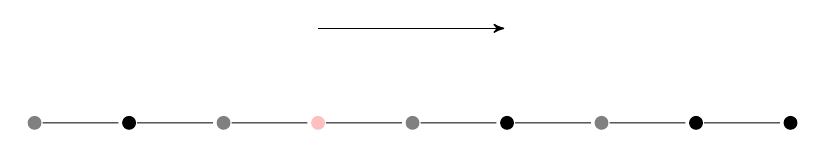
\begin{tikzpicture}[scale=0.6,->,>=stealth',shorten >=1pt,auto,node distance=3cm,
    thick,main node/.style={circle,draw,font=\footnotesize}, small node/.style={circle,font=\footnotesize,inner sep=0pt,minimum size=5pt}]   
   \begin{scope}%[xshift=10cm]
     \node[small node,fill=gray] (b) at (2,5) {};
      \node[small node,fill=black] (c) at (4,5) {};
      %\node[inner sep=0pt]  (d) at (6,5) {\includegraphics[width=.03\textwidth,right]{robot1.jpg}};
      \node[small node,fill=gray] (d) at (6,5) {};
      \node[small node,fill=pink] (e) at (8,5) {};    
      \node[small node,fill=gray]  (f) at (10,5) {};
      %\node[small node,fill=pink]  at (10,5) {};
      \node[small node,fill=black] (i) at (12,5) {};
      \node[small node,fill=gray] (j) at (14,5) {};
      \node[small node,fill=black] (k) at (16,5) {};
      \node[small node,fill=black] (l) at (18,5) {};
      %\node[small node,fill=gray] (m) at (20,5) {};
       \path[-,line width=0.3pt] (b) edge (c);
       \path[-,line width=0.3pt] (c) edge (d);
       \path[-,line width=0.3pt]  (d) edge (e);
      \path[-,line width=0.3pt] (e) edge (f);
      \path[-,line width=0.3pt] (f) edge (i);
      \path[-,line width=0.3pt] (i) edge (j);
      \path[-,line width=0.3pt] (j) edge (k);
      \path[-,line width=0.3pt] (k) edge (l);
      \path[->, line width=0.5pt] (8,7) edge (12,7);
      %\path[-,line width=0.3pt] (l) edge (m);
      %\path[-,line width=0.3pt, color=pink] (f) edge [bend left,-] (8.8,6.8);       
    \end{scope}
  \end{tikzpicture} \\
\end{frame}
\begin{frame}{Subproblem 1: Setup Phase}
 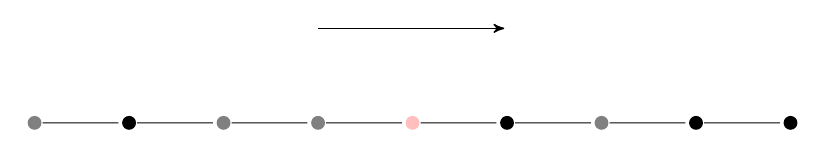
\begin{tikzpicture}[scale=0.6,->,>=stealth',shorten >=1pt,auto,node distance=3cm,
    thick,main node/.style={circle,draw,font=\footnotesize}, small node/.style={circle,font=\footnotesize,inner sep=0pt,minimum size=5pt}]   
   \begin{scope}%[xshift=10cm]
     \node[small node,fill=gray] (b) at (2,5) {};
      \node[small node,fill=black] (c) at (4,5) {};
      %\node[inner sep=0pt]  (d) at (6,5) {\includegraphics[width=.03\textwidth,right]{robot1.jpg}};
      \node[small node,fill=gray] (d) at (6,5) {};
      \node[small node,fill=gray] (e) at (8,5) {};    
      \node[small node,fill=pink]  (f) at (10,5) {};
      %\node[small node,fill=pink]  at (10,5) {};
      \node[small node,fill=black] (i) at (12,5) {};
      \node[small node,fill=gray] (j) at (14,5) {};
      \node[small node,fill=black] (k) at (16,5) {};
      \node[small node,fill=black] (l) at (18,5) {};
      %\node[small node,fill=gray] (m) at (20,5) {};
       \path[-,line width=0.3pt] (b) edge (c);
       \path[-,line width=0.3pt] (c) edge (d);
       \path[-,line width=0.3pt]  (d) edge (e);
      \path[-,line width=0.3pt] (e) edge (f);
      \path[-,line width=0.3pt] (f) edge (i);
      \path[-,line width=0.3pt] (i) edge (j);
      \path[-,line width=0.3pt] (j) edge (k);
      \path[-,line width=0.3pt] (k) edge (l);
      \path[->, line width=0.5pt] (8,7) edge (12,7);
      %\path[-,line width=0.3pt] (l) edge (m);
      %\path[-,line width=0.3pt, color=pink] (f) edge [bend left,-] (8.8,6.8);       
    \end{scope}
  \end{tikzpicture} \\
\end{frame}
\begin{frame}{Subproblem 1: Setup Phase}
 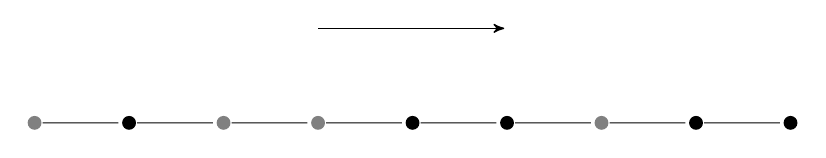
\begin{tikzpicture}[scale=0.6,->,>=stealth',shorten >=1pt,auto,node distance=3cm,
    thick,main node/.style={circle,draw,font=\footnotesize}, small node/.style={circle,font=\footnotesize,inner sep=0pt,minimum size=5pt}]   
   \begin{scope}%[xshift=10cm]
     \node[small node,fill=gray] (b) at (2,5) {};
      \node[small node,fill=black] (c) at (4,5) {};
      %\node[inner sep=0pt]  (d) at (6,5) {\includegraphics[width=.03\textwidth,right]{robot1.jpg}};
      \node[small node,fill=gray] (d) at (6,5) {};
      \node[small node,fill=gray] (e) at (8,5) {};    
      \node[small node,fill=black]  (f) at (10,5) {};
      %\node[small node,fill=pink]  at (10,5) {};
      \node[small node,fill=black] (i) at (12,5) {};
      \node[small node,fill=gray] (j) at (14,5) {};
      \node[small node,fill=black] (k) at (16,5) {};
      \node[small node,fill=black] (l) at (18,5) {};
      %\node[small node,fill=gray] (m) at (20,5) {};
       \path[-,line width=0.3pt] (b) edge (c);
       \path[-,line width=0.3pt] (c) edge (d);
       \path[-,line width=0.3pt]  (d) edge (e);
      \path[-,line width=0.3pt] (e) edge (f);
      \path[-,line width=0.3pt] (f) edge (i);
      \path[-,line width=0.3pt] (i) edge (j);
      \path[-,line width=0.3pt] (j) edge (k);
      \path[-,line width=0.3pt] (k) edge (l);
      \path[->, line width=0.5pt] (8,7) edge (12,7);
      %\path[-,line width=0.3pt] (l) edge (m);
      %\path[-,line width=0.3pt, color=pink] (f) edge [bend left,-] (8.8,6.8);       
    \end{scope}
  \end{tikzpicture} \\
\end{frame}
\begin{frame}{Subproblem 1: Setup Phase}
 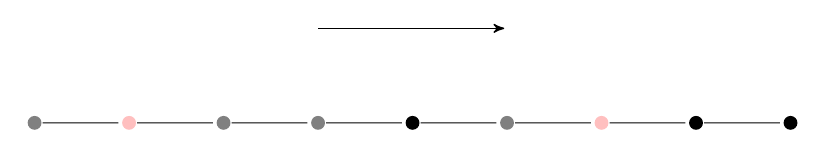
\begin{tikzpicture}[scale=0.6,->,>=stealth',shorten >=1pt,auto,node distance=3cm,
    thick,main node/.style={circle,draw,font=\footnotesize}, small node/.style={circle,font=\footnotesize,inner sep=0pt,minimum size=5pt}]   
   \begin{scope}%[xshift=10cm]
     \node[small node,fill=gray] (b) at (2,5) {};
      \node[small node,fill=pink] (c) at (4,5) {};
      %\node[inner sep=0pt]  (d) at (6,5) {\includegraphics[width=.03\textwidth,right]{robot1.jpg}};
      \node[small node,fill=gray] (d) at (6,5) {};
      \node[small node,fill=gray] (e) at (8,5) {};    
      \node[small node,fill=black]  (f) at (10,5) {};
      %\node[small node,fill=pink]  at (10,5) {};
      \node[small node,fill=gray] (i) at (12,5) {};
      \node[small node,fill=pink] (j) at (14,5) {};
      \node[small node,fill=black] (k) at (16,5) {};
      \node[small node,fill=black] (l) at (18,5) {};
      %\node[small node,fill=gray] (m) at (20,5) {};
       \path[-,line width=0.3pt] (b) edge (c);
       \path[-,line width=0.3pt] (c) edge (d);
       \path[-,line width=0.3pt]  (d) edge (e);
      \path[-,line width=0.3pt] (e) edge (f);
      \path[-,line width=0.3pt] (f) edge (i);
      \path[-,line width=0.3pt] (i) edge (j);
      \path[-,line width=0.3pt] (j) edge (k);
      \path[-,line width=0.3pt] (k) edge (l);
      \path[->, line width=0.5pt] (8,7) edge (12,7);
      %\path[-,line width=0.3pt] (l) edge (m);
      %\path[-,line width=0.3pt, color=pink] (f) edge [bend left,-] (8.8,6.8);       
    \end{scope}
  \end{tikzpicture} \\
\end{frame}
\begin{frame}{Subproblem 1: Setup Phase}
 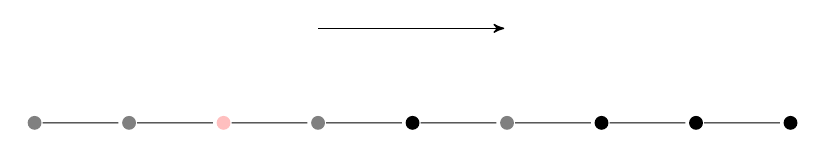
\begin{tikzpicture}[scale=0.6,->,>=stealth',shorten >=1pt,auto,node distance=3cm,
    thick,main node/.style={circle,draw,font=\footnotesize}, small node/.style={circle,font=\footnotesize,inner sep=0pt,minimum size=5pt}]   
   \begin{scope}%[xshift=10cm]
     \node[small node,fill=gray] (b) at (2,5) {};
      \node[small node,fill=gray] (c) at (4,5) {};
      %\node[inner sep=0pt]  (d) at (6,5) {\includegraphics[width=.03\textwidth,right]{robot1.jpg}};
      \node[small node,fill=pink] (d) at (6,5) {};
      \node[small node,fill=gray] (e) at (8,5) {};    
      \node[small node,fill=black]  (f) at (10,5) {};
      %\node[small node,fill=pink]  at (10,5) {};
      \node[small node,fill=gray] (i) at (12,5) {};
      \node[small node,fill=black] (j) at (14,5) {};
      \node[small node,fill=black] (k) at (16,5) {};
      \node[small node,fill=black] (l) at (18,5) {};
      %\node[small node,fill=gray] (m) at (20,5) {};
       \path[-,line width=0.3pt] (b) edge (c);
       \path[-,line width=0.3pt] (c) edge (d);
       \path[-,line width=0.3pt]  (d) edge (e);
      \path[-,line width=0.3pt] (e) edge (f);
      \path[-,line width=0.3pt] (f) edge (i);
      \path[-,line width=0.3pt] (i) edge (j);
      \path[-,line width=0.3pt] (j) edge (k);
      \path[-,line width=0.3pt] (k) edge (l);
      \path[->, line width=0.5pt] (8,7) edge (12,7);
      %\path[-,line width=0.3pt] (l) edge (m);
      %\path[-,line width=0.3pt, color=pink] (f) edge [bend left,-] (8.8,6.8);       
    \end{scope}
  \end{tikzpicture} \\
\end{frame}
\begin{frame}{Subproblem 1: Setup Phase}
 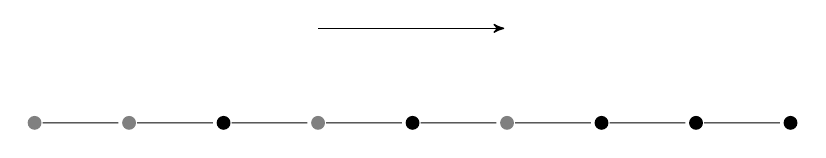
\begin{tikzpicture}[scale=0.6,->,>=stealth',shorten >=1pt,auto,node distance=3cm,
    thick,main node/.style={circle,draw,font=\footnotesize}, small node/.style={circle,font=\footnotesize,inner sep=0pt,minimum size=5pt}]   
   \begin{scope}%[xshift=10cm]
     \node[small node,fill=gray] (b) at (2,5) {};
      \node[small node,fill=gray] (c) at (4,5) {};
      %\node[inner sep=0pt]  (d) at (6,5) {\includegraphics[width=.03\textwidth,right]{robot1.jpg}};
      \node[small node,fill=black] (d) at (6,5) {};
      \node[small node,fill=gray] (e) at (8,5) {};    
      \node[small node,fill=black]  (f) at (10,5) {};
      %\node[small node,fill=pink]  at (10,5) {};
      \node[small node,fill=gray] (i) at (12,5) {};
      \node[small node,fill=black] (j) at (14,5) {};
      \node[small node,fill=black] (k) at (16,5) {};
      \node[small node,fill=black] (l) at (18,5) {};
      %\node[small node,fill=gray] (m) at (20,5) {};
       \path[-,line width=0.3pt] (b) edge (c);
       \path[-,line width=0.3pt] (c) edge (d);
       \path[-,line width=0.3pt]  (d) edge (e);
      \path[-,line width=0.3pt] (e) edge (f);
      \path[-,line width=0.3pt] (f) edge (i);
      \path[-,line width=0.3pt] (i) edge (j);
      \path[-,line width=0.3pt] (j) edge (k);
      \path[-,line width=0.3pt] (k) edge (l);
      \path[->, line width=0.5pt] (8,7) edge (12,7);
      %\path[-,line width=0.3pt] (l) edge (m);
      %\path[-,line width=0.3pt, color=pink] (f) edge [bend left,-] (8.8,6.8);       
    \end{scope}
  \end{tikzpicture} \\
\end{frame}
\begin{frame}{Subproblem 1: Setup Phase}
 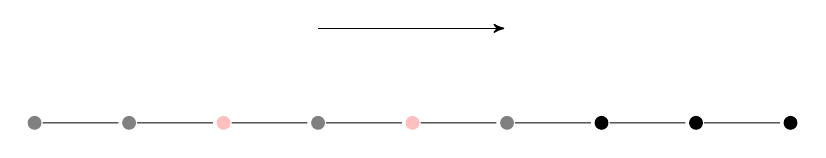
\begin{tikzpicture}[scale=0.6,->,>=stealth',shorten >=1pt,auto,node distance=3cm,
    thick,main node/.style={circle,draw,font=\footnotesize}, small node/.style={circle,font=\footnotesize,inner sep=0pt,minimum size=5pt}]   
   \begin{scope}%[xshift=10cm]
     \node[small node,fill=gray] (b) at (2,5) {};
      \node[small node,fill=gray] (c) at (4,5) {};
      %\node[inner sep=0pt]  (d) at (6,5) {\includegraphics[width=.03\textwidth,right]{robot1.jpg}};
      \node[small node,fill=pink] (d) at (6,5) {};
      \node[small node,fill=gray] (e) at (8,5) {};    
      \node[small node,fill=pink]  (f) at (10,5) {};
      %\node[small node,fill=pink]  at (10,5) {};
      \node[small node,fill=gray] (i) at (12,5) {};
      \node[small node,fill=black] (j) at (14,5) {};
      \node[small node,fill=black] (k) at (16,5) {};
      \node[small node,fill=black] (l) at (18,5) {};
      %\node[small node,fill=gray] (m) at (20,5) {};
       \path[-,line width=0.3pt] (b) edge (c);
       \path[-,line width=0.3pt] (c) edge (d);
       \path[-,line width=0.3pt]  (d) edge (e);
      \path[-,line width=0.3pt] (e) edge (f);
      \path[-,line width=0.3pt] (f) edge (i);
      \path[-,line width=0.3pt] (i) edge (j);
      \path[-,line width=0.3pt] (j) edge (k);
      \path[-,line width=0.3pt] (k) edge (l);
      \path[->, line width=0.5pt] (8,7) edge (12,7);
      %\path[-,line width=0.3pt] (l) edge (m);
      %\path[-,line width=0.3pt, color=pink] (f) edge [bend left,-] (8.8,6.8);       
    \end{scope}
  \end{tikzpicture} \\
\end{frame}
\begin{frame}{Subproblem 1: Setup Phase}
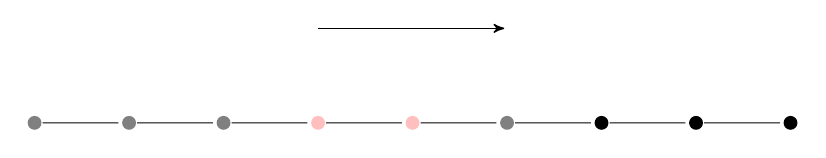
\begin{tikzpicture}[scale=0.6,->,>=stealth',shorten >=1pt,auto,node distance=3cm,
    thick,main node/.style={circle,draw,font=\footnotesize}, small node/.style={circle,font=\footnotesize,inner sep=0pt,minimum size=5pt}]   
   \begin{scope}%[xshift=10cm]
     \node[small node,fill=gray] (b) at (2,5) {};
      \node[small node,fill=gray] (c) at (4,5) {};
      %\node[inner sep=0pt]  (d) at (6,5) {\includegraphics[width=.03\textwidth,right]{robot1.jpg}};
      \node[small node,fill=gray] (d) at (6,5) {};
      \node[small node,fill=pink] (e) at (8,5) {};    
      \node[small node,fill=pink]  (f) at (10,5) {};
      %\node[small node,fill=pink]  at (10,5) {};
      \node[small node,fill=gray] (i) at (12,5) {};
      \node[small node,fill=black] (j) at (14,5) {};
      \node[small node,fill=black] (k) at (16,5) {};
      \node[small node,fill=black] (l) at (18,5) {};
      %\node[small node,fill=gray] (m) at (20,5) {};
       \path[-,line width=0.3pt] (b) edge (c);
       \path[-,line width=0.3pt] (c) edge (d);
       \path[-,line width=0.3pt]  (d) edge (e);
      \path[-,line width=0.3pt] (e) edge (f);
      \path[-,line width=0.3pt] (f) edge (i);
      \path[-,line width=0.3pt] (i) edge (j);
      \path[-,line width=0.3pt] (j) edge (k);
      \path[-,line width=0.3pt] (k) edge (l);
      \path[->, line width=0.5pt] (8,7) edge (12,7);
      %\path[-,line width=0.3pt] (l) edge (m);
      %\path[-,line width=0.3pt, color=pink] (f) edge [bend left,-] (8.8,6.8);       
    \end{scope}
  \end{tikzpicture} \\
\end{frame}
\begin{frame}{Subproblem 1: Setup Phase}
 \begin{tikzpicture}[scale=0.6,->,>=stealth',shorten >=1pt,auto,node distance=3cm,
    thick,main node/.style={circle,draw,font=\footnotesize}, small node/.style={circle,font=\footnotesize,inner sep=0pt,minimum size=5pt}]   
   \begin{scope}%[xshift=10cm]
     \node[small node,fill=gray] (b) at (2,5) {};
      \node[small node,fill=gray] (c) at (4,5) {};
      %\node[inner sep=0pt]  (d) at (6,5) {\includegraphics[width=.03\textwidth,right]{robot1.jpg}};
      \node[small node,fill=gray] (d) at (6,5) {};
      \node[small node,fill=black] (e) at (8,5) {};    
      \node[small node,fill=gray]  (f) at (10,5) {};
      %\node[small node,fill=pink]  at (10,5) {};
      \node[small node,fill=pink] (i) at (12,5) {};
      \node[small node,fill=black] (j) at (14,5) {};
      \node[small node,fill=black] (k) at (16,5) {};
      \node[small node,fill=black] (l) at (18,5) {};
      %\node[small node,fill=gray] (m) at (20,5) {};
       \path[-,line width=0.3pt] (b) edge (c);
       \path[-,line width=0.3pt] (c) edge (d);
       \path[-,line width=0.3pt]  (d) edge (e);
      \path[-,line width=0.3pt] (e) edge (f);
      \path[-,line width=0.3pt] (f) edge (i);
      \path[-,line width=0.3pt] (i) edge (j);
      \path[-,line width=0.3pt] (j) edge (k);
      \path[-,line width=0.3pt] (k) edge (l);
      \path[->, line width=0.5pt] (8,7) edge (12,7);
      %\path[-,line width=0.3pt] (l) edge (m);
      %\path[-,line width=0.3pt, color=pink] (f) edge [bend left,-] (8.8,6.8);       
    \end{scope}
  \end{tikzpicture} \\
\end{frame}
\begin{frame}{Subproblem 1: Setup Phase}
 \begin{tikzpicture}[scale=0.6,->,>=stealth',shorten >=1pt,auto,node distance=3cm,
    thick,main node/.style={circle,draw,font=\footnotesize}, small node/.style={circle,font=\footnotesize,inner sep=0pt,minimum size=5pt}]   
   \begin{scope}%[xshift=10cm]
     \node[small node,fill=gray] (b) at (2,5) {};
      \node[small node,fill=gray] (c) at (4,5) {};
      %\node[inner sep=0pt]  (d) at (6,5) {\includegraphics[width=.03\textwidth,right]{robot1.jpg}};
      \node[small node,fill=gray] (d) at (6,5) {};
      \node[small node,fill=pink] (e) at (8,5) {};    
      \node[small node,fill=gray]  (f) at (10,5) {};
      %\node[small node,fill=pink]  at (10,5) {};
      \node[small node,fill=pink] (i) at (12,5) {};
      \node[small node,fill=black] (j) at (14,5) {};
      \node[small node,fill=black] (k) at (16,5) {};
      \node[small node,fill=black] (l) at (18,5) {};
      %\node[small node,fill=gray] (m) at (20,5) {};
       \path[-,line width=0.3pt] (b) edge (c);
       \path[-,line width=0.3pt] (c) edge (d);
       \path[-,line width=0.3pt]  (d) edge (e);
      \path[-,line width=0.3pt] (e) edge (f);
      \path[-,line width=0.3pt] (f) edge (i);
      \path[-,line width=0.3pt] (i) edge (j);
      \path[-,line width=0.3pt] (j) edge (k);
      \path[-,line width=0.3pt] (k) edge (l);
      \path[->, line width=0.5pt] (8,7) edge (12,7);
      %\path[-,line width=0.3pt] (l) edge (m);
      %\path[-,line width=0.3pt, color=pink] (f) edge [bend left,-] (8.8,6.8);       
    \end{scope}
  \end{tikzpicture} \\
\end{frame}
\begin{frame}{Subproblem 1: Setup Phase}
 \begin{tikzpicture}[scale=0.6,->,>=stealth',shorten >=1pt,auto,node distance=3cm,
    thick,main node/.style={circle,draw,font=\footnotesize}, small node/.style={circle,font=\footnotesize,inner sep=0pt,minimum size=5pt}]   
   \begin{scope}%[xshift=10cm]
     \node[small node,fill=gray] (b) at (2,5) {};
      \node[small node,fill=gray] (c) at (4,5) {};
      %\node[inner sep=0pt]  (d) at (6,5) {\includegraphics[width=.03\textwidth,right]{robot1.jpg}};
      \node[small node,fill=gray] (d) at (6,5) {};
      \node[small node,fill=gray] (e) at (8,5) {};    
      \node[small node,fill=pink]  (f) at (10,5) {};
      %\node[small node,fill=pink]  at (10,5) {};
      \node[small node,fill=black] (i) at (12,5) {};
      \node[small node,fill=black] (j) at (14,5) {};
      \node[small node,fill=black] (k) at (16,5) {};
      \node[small node,fill=black] (l) at (18,5) {};
      %\node[small node,fill=gray] (m) at (20,5) {};
       \path[-,line width=0.3pt] (b) edge (c);
       \path[-,line width=0.3pt] (c) edge (d);
       \path[-,line width=0.3pt]  (d) edge (e);
      \path[-,line width=0.3pt] (e) edge (f);
      \path[-,line width=0.3pt] (f) edge (i);
      \path[-,line width=0.3pt] (i) edge (j);
      \path[-,line width=0.3pt] (j) edge (k);
      \path[-,line width=0.3pt] (k) edge (l);
      \path[->, line width=0.5pt] (8,7) edge (12,7);
      %\path[-,line width=0.3pt] (l) edge (m);
      %\path[-,line width=0.3pt, color=pink] (f) edge [bend left,-] (8.8,6.8);       
    \end{scope}
  \end{tikzpicture} \\
\end{frame}
\begin{frame}{Subproblem 1: Setup Phase}
 \begin{tikzpicture}[scale=0.6,->,>=stealth',shorten >=1pt,auto,node distance=3cm,
    thick,main node/.style={circle,draw,font=\footnotesize}, small node/.style={circle,font=\footnotesize,inner sep=0pt,minimum size=5pt}]   
   \begin{scope}%[xshift=10cm]
     \node[small node,fill=gray] (b) at (2,5) {};
      \node[small node,fill=gray] (c) at (4,5) {};
      %\node[inner sep=0pt]  (d) at (6,5) {\includegraphics[width=.03\textwidth,right]{robot1.jpg}};
      \node[small node,fill=gray] (d) at (6,5) {};
      \node[small node,fill=gray] (e) at (8,5) {};    
      \node[small node,fill=black]  (f) at (10,5) {};
      %\node[small node,fill=pink]  at (10,5) {};
      \node[small node,fill=black] (i) at (12,5) {};
      \node[small node,fill=black] (j) at (14,5) {};
      \node[small node,fill=black] (k) at (16,5) {};
      \node[small node,fill=black] (l) at (18,5) {};
      %\node[small node,fill=gray] (m) at (20,5) {};
       \path[-,line width=0.3pt] (b) edge (c);
       \path[-,line width=0.3pt] (c) edge (d);
       \path[-,line width=0.3pt]  (d) edge (e);
      \path[-,line width=0.3pt] (e) edge (f);
      \path[-,line width=0.3pt] (f) edge (i);
      \path[-,line width=0.3pt] (i) edge (j);
      \path[-,line width=0.3pt] (j) edge (k);
      \path[-,line width=0.3pt] (k) edge (l);
      \path[->, line width=0.5pt] (8,7) edge (12,7);
      %\path[-,line width=0.3pt] (l) edge (m);
      %\path[-,line width=0.3pt, color=pink] (f) edge [bend left,-] (8.8,6.8);       
    \end{scope}
  \end{tikzpicture} \\
\end{frame}
%
%
%%%%%%%%%%%%%%%%%%%%%%%%%%%%%%%%%%%%%%%%%%%%%%%%%%%%%%%
%%%%%%%%%%%%%%%%%%%%%%%%%%%%%%%%%%%%%%%%%%%%%%%%%%%%%%%
\miniframeson
\subsection{subproblem 2}

\begin{frame}{Subproblem 2: Line Exploration}
 \begin{tikzpicture}[scale=0.6,->,>=stealth',shorten >=1pt,auto,node distance=3cm,
    thick,main node/.style={circle,draw,font=\footnotesize}, small node/.style={circle,font=\footnotesize,inner sep=0pt,minimum size=5pt}]   
     \begin{scope}[yshift=-3cm]
     \node[small node,fill=black] (b) at (2,5) {};
      \node[small node,fill=black] (c) at (4,5) {};
      %\node[inner sep=0pt]  (d) at (6,5) {\includegraphics[width=.03\textwidth,right]{robot1.jpg}};
       \node[small node,fill=black] (d) at (6,5) {};
       \node[small node,fill=black] (e) at (8,5) {};    
      \node[small node,fill=black]  (f) at (10,5) {};
      %\node[small node,fill=pink]  at (10,5) {};
      \node[small node,fill=gray] (i) at (12,5) {};
      \node[small node,fill=gray] (j) at (14,5) {};
      \node[small node,fill=gray] (k) at (16,5) {};
      \node[small node,fill=gray] (l) at (18,5) {};
      %\node[small node,fill=gray] (m) at (20,5) {};
       \path[-,line width=0.3pt] (b) edge (c);
       \path[-,line width=0.3pt] (c) edge (d);
       \path[-,line width=0.3pt]  (d) edge (e);
      \path[-,line width=0.3pt] (e) edge (f);
      \path[-,line width=0.3pt] (f) edge (i);
      \path[-,line width=0.3pt] (i) edge (j);
      \path[-,line width=0.3pt] (j) edge (k);
      \path[-,line width=0.3pt] (k) edge (l);
      %\path[-,line width=0.3pt] (l) edge (m);
      %\path[-,line width=0.3pt, color=pink] (f) edge [bend left,-] (8.8,6.8);   
    \end{scope}
  \end{tikzpicture} 
\end{frame}
\miniframesoff
\begin{frame}{Subproblem 2: Line Exploration}
 \begin{tikzpicture}[scale=0.6,->,>=stealth',shorten >=1pt,auto,node distance=3cm,
    thick,main node/.style={circle,draw,font=\footnotesize}, small node/.style={circle,font=\footnotesize,inner sep=0pt,minimum size=5pt}]   
     \begin{scope}[yshift=-3cm]
     \node[small node,fill=black] (b) at (2,5) {};
      \node[small node,fill=black] (c) at (4,5) {};
      %\node[inner sep=0pt]  (d) at (6,5) {\includegraphics[width=.03\textwidth,right]{robot1.jpg}};
       \node[small node,fill=black] (d) at (6,5) {};
       \node[small node,fill=black] (e) at (8,5) {};    
      \node[small node,fill=black]  (f) at (10,5) {};
      %\node[small node,fill=pink]  at (10,5) {};
      \node[small node,fill=gray] (i) at (12,5) {};
      \node[small node,fill=gray] (j) at (14,5) {};
      \node[small node,fill=gray] (k) at (16,5) {};
      \node[small node,fill=gray] (l) at (18,5) {};
      %\node[small node,fill=gray] (m) at (20,5) {};
       \path[-,line width=0.3pt] (b) edge (c);
       \path[-,line width=0.3pt] (c) edge (d);
       \path[-,line width=0.3pt]  (d) edge (e);
      \path[-,line width=0.3pt] (e) edge (f);
      \path[-,line width=0.3pt] (f) edge (i);
      \path[-,line width=0.3pt] (i) edge (j);
      \path[-,line width=0.3pt] (j) edge (k);
      \path[-,line width=0.3pt] (k) edge (l);
      %\path[-,line width=0.3pt] (l) edge (m);
      %\path[-,line width=0.3pt, color=pink] (f) edge [bend left,-] (8.8,6.8);       
    \end{scope}
  \end{tikzpicture} 
    \\[0.5in]  
    \begin{itemize}
     \item Starting from consecutive configuration, explore the line and stop.
     \item $n$ odd, $\# robots$ odd
    \end{itemize}  
\end{frame}

\begin{frame}{Actual Line Exploration}
 \begin{tikzpicture}[scale=0.6,->,>=stealth',shorten >=1pt,auto,node distance=3cm,
    thick,main node/.style={circle,draw,font=\footnotesize}, small node/.style={circle,font=\footnotesize,inner sep=0pt,minimum size=5pt}]   
     \begin{scope}[yshift=-3cm]
     \node[small node,fill=black] (b) at (2,5) {};
      \node[small node,fill=orange] (c) at (4,5) {};
      %\node[inner sep=0pt]  (d) at (6,5) {\includegraphics[width=.03\textwidth,right]{robot1.jpg}};
       \node[small node,fill=black] (d) at (6,5) {};
       \node[small node,fill=black] (e) at (8,5) {};    
      \node[small node,fill=black]  (f) at (10,5) {};
      %\node[small node,fill=pink]  at (10,5) {};
      \node[small node,fill=gray] (i) at (12,5) {};
      \node[small node,fill=gray] (j) at (14,5) {};
      \node[small node,fill=gray] (k) at (16,5) {};
      \node[small node,fill=gray] (l) at (18,5) {};
      %\node[small node,fill=gray] (m) at (20,5) {};
       \path[-,line width=0.3pt] (b) edge (c);
       \path[-,line width=0.3pt] (c) edge (d);
       \path[-,line width=0.3pt]  (d) edge (e);
      \path[-,line width=0.3pt] (e) edge (f);
      \path[-,line width=0.3pt] (f) edge (i);
      \path[-,line width=0.3pt] (i) edge (j);
      \path[-,line width=0.3pt] (j) edge (k);
      \path[-,line width=0.3pt] (k) edge (l);
      %\path[-,line width=0.3pt] (l) edge (m);
      %\path[-,line width=0.3pt, color=pink] (f) edge [bend left,-] (8.8,6.8);       
    \end{scope}
  \end{tikzpicture} 
  \\[0.5in]  
  \begin{itemize}
     \item Move second robot from the border to the first one.
    \end{itemize} 
\end{frame}
\begin{frame}{Subproblem 2: Exploration Phase}
 \begin{tikzpicture}[scale=0.6,->,>=stealth',shorten >=1pt,auto,node distance=3cm,
    thick,main node/.style={circle,draw,font=\footnotesize}, small node/.style={circle,font=\footnotesize,inner sep=0pt,minimum size=5pt}]   
     \begin{scope}[yshift=-3cm]
     \node[diamond,fill=orange] (b) at (2,5) {};
      \node[small node,fill=gray] (c) at (4,5) {};
      %\node[inner sep=0pt]  (d) at (6,5) {\includegraphics[width=.03\textwidth,right]{robot1.jpg}};
       \node[small node,fill=black] (d) at (6,5) {};
       \node[small node,fill=black] (e) at (8,5) {};    
      \node[small node,fill=black]  (f) at (10,5) {};
      %\node[small node,fill=pink]  at (10,5) {};
      \node[small node,fill=gray] (i) at (12,5) {};
      \node[small node,fill=gray] (j) at (14,5) {};
      \node[small node,fill=gray] (k) at (16,5) {};
      \node[small node,fill=gray] (l) at (18,5) {};
      %\node[small node,fill=gray] (m) at (20,5) {};
       \path[-,line width=0.3pt] (b) edge (c);
       \path[-,line width=0.3pt] (c) edge (d);
       \path[-,line width=0.3pt]  (d) edge (e);
      \path[-,line width=0.3pt] (e) edge (f);
      \path[-,line width=0.3pt] (f) edge (i);
      \path[-,line width=0.3pt] (i) edge (j);
      \path[-,line width=0.3pt] (j) edge (k);
      \path[-,line width=0.3pt] (k) edge (l);
      %\path[-,line width=0.3pt] (l) edge (m);
      %\path[-,line width=0.3pt, color=pink] (f) edge [bend left,-] (8.8,6.8);       
    \end{scope}
  \end{tikzpicture} 
  \\[0.5in]  
  \begin{itemize}
     \item Move second robot from the border to the first one.
    \end{itemize} 
\end{frame}
\begin{frame}{Subproblem 2: Exploration Phase}
 \begin{tikzpicture}[scale=0.6,->,>=stealth',shorten >=1pt,auto,node distance=3cm,
    thick,main node/.style={circle,draw,font=\footnotesize}, small node/.style={circle,font=\footnotesize,inner sep=0pt,minimum size=5pt}]   
     \begin{scope}[yshift=-3cm]
     \node[diamond,fill=black] (b) at (2,5) {};
      \node[small node,fill=gray] (c) at (4,5) {};
      %\node[inner sep=0pt]  (d) at (6,5) {\includegraphics[width=.03\textwidth,right]{robot1.jpg}};
       \node[small node,fill=black] (d) at (6,5) {};
       \node[small node,fill=black] (e) at (8,5) {};    
      \node[small node,fill=black]  (f) at (10,5) {};
      %\node[small node,fill=pink]  at (10,5) {};
      \node[small node,fill=gray] (i) at (12,5) {};
      \node[small node,fill=gray] (j) at (14,5) {};
      \node[small node,fill=gray] (k) at (16,5) {};
      \node[small node,fill=gray] (l) at (18,5) {};
      %\node[small node,fill=gray] (m) at (20,5) {};
       \path[-,line width=0.3pt] (b) edge (c);
       \path[-,line width=0.3pt] (c) edge (d);
       \path[-,line width=0.3pt]  (d) edge (e);
      \path[-,line width=0.3pt] (e) edge (f);
      \path[-,line width=0.3pt] (f) edge (i);
      \path[-,line width=0.3pt] (i) edge (j);
      \path[-,line width=0.3pt] (j) edge (k);
      \path[-,line width=0.3pt] (k) edge (l);
      %\path[-,line width=0.3pt] (l) edge (m);
      %\path[-,line width=0.3pt, color=pink] (f) edge [bend left,-] (8.8,6.8);       
    \end{scope}
  \end{tikzpicture} 
  \\[0.5in]  
  \begin{itemize}
     \item Move second robot from the border to the first one. \\
     \textcolor{orange}{Exploration Phase}
    \end{itemize} 
\end{frame}
\begin{frame}{Subproblem 2: Exploration Phase}
 \begin{tikzpicture}[scale=0.6,->,>=stealth',shorten >=1pt,auto,node distance=3cm,
    thick,main node/.style={circle,draw,font=\footnotesize}, small node/.style={circle,font=\footnotesize,inner sep=0pt,minimum size=5pt}]   
     \begin{scope}[yshift=-3cm]
     \node[diamond,fill=black] (b) at (2,5) {};
      \node[small node,fill=gray] (c) at (4,5) {};
      %\node[inner sep=0pt]  (d) at (6,5) {\includegraphics[width=.03\textwidth,right]{robot1.jpg}};
       \node[small node,fill=black] (d) at (6,5) {};
       \node[small node,fill=black] (e) at (8,5) {};    
      \node[small node,fill=orange]  (f) at (10,5) {};
      %\node[small node,fill=pink]  at (10,5) {};
      \node[small node,fill=gray] (i) at (12,5) {};
      \node[small node,fill=gray] (j) at (14,5) {};
      \node[small node,fill=gray] (k) at (16,5) {};
      \node[small node,fill=gray] (l) at (18,5) {};
      %\node[small node,fill=gray] (m) at (20,5) {};
       \path[-,line width=0.3pt] (b) edge (c);
       \path[-,line width=0.3pt] (c) edge (d);
       \path[-,line width=0.3pt]  (d) edge (e);
      \path[-,line width=0.3pt] (e) edge (f);
      \path[-,line width=0.3pt] (f) edge (i);
      \path[-,line width=0.3pt] (i) edge (j);
      \path[-,line width=0.3pt] (j) edge (k);
      \path[-,line width=0.3pt] (k) edge (l);
      %\path[-,line width=0.3pt] (l) edge (m);
      %\path[-,line width=0.3pt, color=pink] (f) edge [bend left,-] (8.8,6.8);       
    \end{scope}
  \end{tikzpicture} 
  \\[0.5in]  
  \begin{itemize}
     \item Move second robot from the border to the first one. \\
     \textcolor{orange}{Exploration Phase}
     \item Move external robot along the line.
    \end{itemize} 
\end{frame}
\begin{frame}{Subproblem 2: Exploration Phase}
 \begin{tikzpicture}[scale=0.6,->,>=stealth',shorten >=1pt,auto,node distance=3cm,
    thick,main node/.style={circle,draw,font=\footnotesize}, small node/.style={circle,font=\footnotesize,inner sep=0pt,minimum size=5pt}]   
     \begin{scope}[yshift=-3cm]
     \node[diamond,fill=black] (b) at (2,5) {};
      \node[small node,fill=gray] (c) at (4,5) {};
      %\node[inner sep=0pt]  (d) at (6,5) {\includegraphics[width=.03\textwidth,right]{robot1.jpg}};
       \node[small node,fill=black] (d) at (6,5) {};
       \node[small node,fill=black] (e) at (8,5) {};    
      \node[small node,fill=gray]  (f) at (10,5) {};
      %\node[small node,fill=pink]  at (10,5) {};
      \node[small node,fill=orange] (i) at (12,5) {};
      \node[small node,fill=gray] (j) at (14,5) {};
      \node[small node,fill=gray] (k) at (16,5) {};
      \node[small node,fill=gray] (l) at (18,5) {};
      %\node[small node,fill=gray] (m) at (20,5) {};
       \path[-,line width=0.3pt] (b) edge (c);
       \path[-,line width=0.3pt] (c) edge (d);
       \path[-,line width=0.3pt]  (d) edge (e);
      \path[-,line width=0.3pt] (e) edge (f);
      \path[-,line width=0.3pt] (f) edge (i);
      \path[-,line width=0.3pt] (i) edge (j);
      \path[-,line width=0.3pt] (j) edge (k);
      \path[-,line width=0.3pt] (k) edge (l);
      %\path[-,line width=0.3pt] (l) edge (m);
      %\path[-,line width=0.3pt, color=pink] (f) edge [bend left,-] (8.8,6.8);       
    \end{scope}
  \end{tikzpicture} 
  \\[0.5in]  
  \begin{itemize}
     \item Move second robot from the border to the first one. \\
     \textcolor{orange}{Exploration Phase}
     \item Move external robot along the line.
    \end{itemize} 
\end{frame}
\begin{frame}{Subproblem 2: Exploration Phase}
 \begin{tikzpicture}[scale=0.6,->,>=stealth',shorten >=1pt,auto,node distance=3cm,
    thick,main node/.style={circle,draw,font=\footnotesize}, small node/.style={circle,font=\footnotesize,inner sep=0pt,minimum size=5pt}]   
     \begin{scope}[yshift=-3cm]
     \node[diamond,fill=black] (b) at (2,5) {};
      \node[small node,fill=gray] (c) at (4,5) {};
      %\node[inner sep=0pt]  (d) at (6,5) {\includegraphics[width=.03\textwidth,right]{robot1.jpg}};
       \node[small node,fill=black] (d) at (6,5) {};
       \node[small node,fill=black] (e) at (8,5) {};    
      \node[small node,fill=gray]  (f) at (10,5) {};
      %\node[small node,fill=pink]  at (10,5) {};
      \node[small node,fill=gray] (i) at (12,5) {};
      \node[small node,fill=orange] (j) at (14,5) {};
      \node[small node,fill=gray] (k) at (16,5) {};
      \node[small node,fill=gray] (l) at (18,5) {};
      %\node[small node,fill=gray] (m) at (20,5) {};
       \path[-,line width=0.3pt] (b) edge (c);
       \path[-,line width=0.3pt] (c) edge (d);
       \path[-,line width=0.3pt]  (d) edge (e);
      \path[-,line width=0.3pt] (e) edge (f);
      \path[-,line width=0.3pt] (f) edge (i);
      \path[-,line width=0.3pt] (i) edge (j);
      \path[-,line width=0.3pt] (j) edge (k);
      \path[-,line width=0.3pt] (k) edge (l);
      %\path[-,line width=0.3pt] (l) edge (m);
      %\path[-,line width=0.3pt, color=pink] (f) edge [bend left,-] (8.8,6.8);       
    \end{scope}
  \end{tikzpicture} 
  \\[0.5in]  
  \begin{itemize}
     \item Move second robot from the border to the first one. \\
     \textcolor{orange}{Exploration Phase}
     \item Move external robot along the line.
    \end{itemize} 
\end{frame}
\begin{frame}{Subproblem 2: Exploration Phase}
 \begin{tikzpicture}[scale=0.6,->,>=stealth',shorten >=1pt,auto,node distance=3cm,
    thick,main node/.style={circle,draw,font=\footnotesize}, small node/.style={circle,font=\footnotesize,inner sep=0pt,minimum size=5pt}]   
     \begin{scope}[yshift=-3cm]
     \node[diamond,fill=black] (b) at (2,5) {};
      \node[small node,fill=gray] (c) at (4,5) {};
      %\node[inner sep=0pt]  (d) at (6,5) {\includegraphics[width=.03\textwidth,right]{robot1.jpg}};
       \node[small node,fill=black] (d) at (6,5) {};
       \node[small node,fill=black] (e) at (8,5) {};    
      \node[small node,fill=gray]  (f) at (10,5) {};
      %\node[small node,fill=pink]  at (10,5) {};
      \node[small node,fill=gray] (i) at (12,5) {};
      \node[small node,fill=gray] (j) at (14,5) {};
      \node[small node,fill=orange] (k) at (16,5) {};
      \node[small node,fill=gray] (l) at (18,5) {};
      %\node[small node,fill=gray] (m) at (20,5) {};
       \path[-,line width=0.3pt] (b) edge (c);
       \path[-,line width=0.3pt] (c) edge (d);
       \path[-,line width=0.3pt]  (d) edge (e);
      \path[-,line width=0.3pt] (e) edge (f);
      \path[-,line width=0.3pt] (f) edge (i);
      \path[-,line width=0.3pt] (i) edge (j);
      \path[-,line width=0.3pt] (j) edge (k);
      \path[-,line width=0.3pt] (k) edge (l);
      %\path[-,line width=0.3pt] (l) edge (m);
      %\path[-,line width=0.3pt, color=pink] (f) edge [bend left,-] (8.8,6.8);       
    \end{scope}
  \end{tikzpicture} 
  \\[0.5in]  
  \begin{itemize}
     \item Move second robot from the border to the first one. \\
     \textcolor{orange}{Exploration Phase}
     \item Move external robot along the line.
    \end{itemize} 
\end{frame}
\begin{frame}{Subproblem 2: Exploration Phase}
 \begin{tikzpicture}[scale=0.6,->,>=stealth',shorten >=1pt,auto,node distance=3cm,
    thick,main node/.style={circle,draw,font=\footnotesize}, small node/.style={circle,font=\footnotesize,inner sep=0pt,minimum size=5pt}]   
     \begin{scope}[yshift=-3cm]
     \node[diamond,fill=black] (b) at (2,5) {};
      \node[small node,fill=gray] (c) at (4,5) {};
      %\node[inner sep=0pt]  (d) at (6,5) {\includegraphics[width=.03\textwidth,right]{robot1.jpg}};
       \node[small node,fill=black] (d) at (6,5) {};
       \node[small node,fill=black] (e) at (8,5) {};    
      \node[small node,fill=gray]  (f) at (10,5) {};
      %\node[small node,fill=pink]  at (10,5) {};
      \node[small node,fill=gray] (i) at (12,5) {};
      \node[small node,fill=gray] (j) at (14,5) {};
      \node[small node,fill=gray] (k) at (16,5) {};
      \node[small node,fill=orange] (l) at (18,5) {};
      %\node[small node,fill=gray] (m) at (20,5) {};
       \path[-,line width=0.3pt] (b) edge (c);
       \path[-,line width=0.3pt] (c) edge (d);
       \path[-,line width=0.3pt]  (d) edge (e);
      \path[-,line width=0.3pt] (e) edge (f);
      \path[-,line width=0.3pt] (f) edge (i);
      \path[-,line width=0.3pt] (i) edge (j);
      \path[-,line width=0.3pt] (j) edge (k);
      \path[-,line width=0.3pt] (k) edge (l);
      %\path[-,line width=0.3pt] (l) edge (m);
      %\path[-,line width=0.3pt, color=pink] (f) edge [bend left,-] (8.8,6.8);       
    \end{scope}
  \end{tikzpicture} 
  \\[0.5in]  
  \begin{itemize}
     \item Move second robot from the border to the first one. \\
     \textcolor{orange}{Exploration Phase}
     \item Move external robot along the line.
    \end{itemize} 
\end{frame}
\begin{frame}{Subproblem 2: Exploration Phase}
 \begin{tikzpicture}[scale=0.6,->,>=stealth',shorten >=1pt,auto,node distance=3cm,
    thick,main node/.style={circle,draw,font=\footnotesize}, small node/.style={circle,font=\footnotesize,inner sep=0pt,minimum size=5pt}]   
     \begin{scope}[yshift=-3cm]
     \node[diamond,fill=black] (b) at (2,5) {};
      \node[small node,fill=gray] (c) at (4,5) {};
      %\node[inner sep=0pt]  (d) at (6,5) {\includegraphics[width=.03\textwidth,right]{robot1.jpg}};
       \node[small node,fill=black] (d) at (6,5) {};
       \node[small node,fill=black] (e) at (8,5) {};    
      \node[small node,fill=gray]  (f) at (10,5) {};
      %\node[small node,fill=pink]  at (10,5) {};
      \node[small node,fill=gray] (i) at (12,5) {};
      \node[small node,fill=gray] (j) at (14,5) {};
      \node[small node,fill=gray] (k) at (16,5) {};
      \node[small node,fill=black] (l) at (18,5) {};
      %\node[small node,fill=gray] (m) at (20,5) {};
       \path[-,line width=0.3pt] (b) edge (c);
       \path[-,line width=0.3pt] (c) edge (d);
       \path[-,line width=0.3pt]  (d) edge (e);
      \path[-,line width=0.3pt] (e) edge (f);
      \path[-,line width=0.3pt] (f) edge (i);
      \path[-,line width=0.3pt] (i) edge (j);
      \path[-,line width=0.3pt] (j) edge (k);
      \path[-,line width=0.3pt] (k) edge (l);
      %\path[-,line width=0.3pt] (l) edge (m);
      %\path[-,line width=0.3pt, color=pink] (f) edge [bend left,-] (8.8,6.8);       
    \end{scope}
  \end{tikzpicture} 
  \\[0.5in]  
  \begin{itemize}
     \item Move second robot from the border to the first one. \\
     \textcolor{orange}{Exploration Phase}
     \item Move external robot along the line.     \\
     \textcolor{orange}{Line Explored}
     \item Termination: Exploring robotreaches the other end
    \end{itemize} 
\end{frame}
\miniframeson
\begin{frame}{Line Exploration Problem}
Algorithm : Setup Phase + Exploration Phase
\\[0.3in] 
   \begin{itemize}
     \item Any initial configuration. 
     \item Line explored.
     \item Uniqually identified termination configuraions.
    \end{itemize} 
\end{frame}
\miniframesoff
%%%%%%%%%%%%%%%%%%%%%%%%%%%%%%%%%%%%%%%%%%%%%%%%%%%%%%
%%%%%%%%%%%%%%%%%%%%%%%%%%%%%%%%%%%%%%%%%%%%%%%%%%%%%%
\section{\scshape Results}
\subsection{Frame 1}
\miniframeson
\begin{frame}{Terminal configuration}
Terminal configuration must contain a tower.
\\[0.3in] 
\begin{itemize}
     \item Initial configuration cannot be terminal.
     \item Configurations without towers: potential initial configurations.
    \end{itemize} 
\end{frame}
%\miniframesoff
\begin{frame}{Exploration with 1 robot}
\textcolor{gray}{Terminal configuration must contain a tower.}
\\[0.3in] 
If $k = 1$, then the exploration of the line is impossible. 
\end{frame}
\begin{frame}{Exploration with 2 robots}
If $k = 1$, then the exploration of the line is impossible, even if the robots agree on a common orientation of it. 
\end{frame}
\miniframesoff
\begin{frame}{Exploration with 2 robots}
If $k = 1$, then the exploration of the line is impossible, even if the robots agree on a common orientation of it. 
\\[0.3in] 
Suppose there exists an algorithm A. Let $n\geq3$.


\end{frame}

\begin{frame}{Exploration with 2 robots}
Suppose there exists an algorithm A. Let $n\geq3$.
\\[0.3in]
There exists a finite sequence of configuration:\\
from \textcolor{blue}{\textit{initial configuration} } to \textcolor{brown}{\textit{terminal configuration} }. \\[0.1in]
 \begin{tikzpicture}[scale=0.8,->,>=stealth',shorten >=1pt,auto,node distance=3cm,
    thick,main node/.style={circle,draw,font=\footnotesize}, small node/.style={circle,font=\footnotesize,inner sep=0pt,minimum size=5pt}]   
     \begin{scope}%[yshift=-3cm]
     \node[main node, draw, color=blue](b) at (2,5) {};
      \node[main node,draw] (c) at (4,5) {};
      %\node[inner sep=0pt]  (d) at (6,5) {\includegraphics[width=.03\textwidth,right]{robot1.jpg}};
       \node[main node,draw] (d) at (6,5) {};
       \node[main node,draw] (e) at (8,5) {};    
      \node[main node,draw]  (f) at (10,5) {};
      %\node[small node,fill=pink]  at (10,5) {};
      \node[diamond,draw, color=brown] (i) at (12,5) {};
      %\node[small node,fill=gray] (m) at (20,5) {};
       \path[->,line width=0.3pt] (b) edge [bend left] (c);
       \path[->,line width=0.3pt] (c) edge [bend left] (d);
       \path[-,line width=0.3pt, loosely dotted]  (d) edge  (e);
       %\path[->,line width=0.3pt]  (d) edge [bend left] (e);
      \path[->,line width=0.3pt] (e) edge [bend left] (f);
      \path[->,line width=0.3pt] (f) edge [bend left] (i);
      %\path[-,line width=0.3pt] (l) edge (m);
      %\path[-,line width=0.3pt, color=pink] (f) edge [bend left,-] (8.8,6.8);       
    \end{scope}
  \end{tikzpicture}
\end{frame}
\begin{frame}{Exploration with 2 robots}
Suppose there exists an algorithm A. Let $n\geq3$.
\\[0.3in]
There exists a finite sequence of configuration:\\
from \textcolor{blue}{\textit{initial configuration} } to \textcolor{brown}{\textit{terminal configuration} }. \\[0.1in]
 \begin{tikzpicture}[scale=0.8,->,>=stealth',shorten >=1pt,auto,node distance=3cm,
    thick,main node/.style={circle,draw,font=\footnotesize}, small node/.style={circle,font=\footnotesize,inner sep=0pt,minimum size=5pt}]   
     \begin{scope}%[yshift=-3cm]
     \node[main node, draw, color=blue](b) at (2,5) {};
      \node[main node,draw] (c) at (4,5) {};
      %\node[inner sep=0pt]  (d) at (6,5) {\includegraphics[width=.03\textwidth,right]{robot1.jpg}};
       \node[main node,draw] (d) at (6,5) {};
       \node[main node,draw] (e) at (8,5) {};    
      \node[main node,fill=red]  (f) at (10,5) {};
      %\node[small node,fill=pink]  at (10,5) {};
      \node[diamond,draw, color=brown] (i) at (12,5) {};
      %\node[small node,fill=gray] (m) at (20,5) {};
       \path[->,line width=0.3pt] (b) edge [bend left] (c);
       \path[->,line width=0.3pt] (c) edge [bend left] (d);
       \path[-,line width=0.3pt, loosely dotted]  (d) edge  (e);
       %\path[->,line width=0.3pt]  (d) edge [bend left] (e);
      \path[->,line width=0.3pt] (e) edge [bend left] (f);
      \path[->,line width=0.3pt] (f) edge [bend left] (i);
      %\path[-,line width=0.3pt] (l) edge (m);
      %\path[-,line width=0.3pt, color=pink] (f) edge [bend left,-] (8.8,6.8);       
    \end{scope}
  \end{tikzpicture} \\
  Consider the \textcolor{red}{configuration} preceding the terminal one. \\
  It has no towers, that is, it is a potential initial configuration.
\end{frame}
\begin{frame}{Exploration with 2 robots}
Suppose there exists an algorithm A. Let $n\geq3$.
\\[0.3in]
There exists a finite sequence of configuration:\\
from \textcolor{blue}{\textit{initial configuration} } to \textcolor{brown}{\textit{terminal configuration} }. \\[0.1in]
 \begin{tikzpicture}[scale=0.8,->,>=stealth',shorten >=1pt,auto,node distance=3cm,
    thick,main node/.style={circle,draw,font=\footnotesize}, small node/.style={circle,font=\footnotesize,inner sep=0pt,minimum size=5pt}]   
     \begin{scope}%[yshift=-3cm]
     \node[main node, draw, color=blue](b) at (2,5) {};
      \node[main node,draw] (c) at (4,5) {};
      %\node[inner sep=0pt]  (d) at (6,5) {\includegraphics[width=.03\textwidth,right]{robot1.jpg}};
       \node[main node,draw] (d) at (6,5) {};
       \node[main node,draw] (e) at (8,5) {};    
      \node[main node,draw]  (f) at (10,5) {};
      %\node[small node,fill=pink]  at (10,5) {};
      \node[diamond,draw, color=brown] (i) at (12,5) {};
      %\node[small node,fill=gray] (m) at (20,5) {};
       \path[->,line width=0.3pt] (b) edge [bend left] (c);
       \path[->,line width=0.3pt] (c) edge [bend left] (d);
       \path[-,line width=0.3pt, loosely dotted]  (d) edge  (e);
       %\path[->,line width=0.3pt]  (d) edge [bend left] (e);
      \path[->,line width=0.3pt] (e) edge [bend left] (f);
      \path[->,line width=0.3pt] (f) edge [bend left] (i);
      %\path[-,line width=0.3pt] (l) edge (m);
      %\path[-,line width=0.3pt, color=pink] (f) edge [bend left,-] (8.8,6.8);       
    \end{scope}
     \begin{scope}[yshift=-2cm]
     \node[main node, draw, color=blue](f) at (10,5){};
   
    \end{scope}
  \end{tikzpicture}
\end{frame}

\begin{frame}{Exploration with 2 robots}
There exists a finite sequence of configuration:\\
from \textcolor{blue}{\textit{initial configuration} } to \textcolor{brown}{\textit{terminal configuration} }. \\[0.1in]
 \begin{tikzpicture}[scale=0.8,->,>=stealth',shorten >=1pt,auto,node distance=3cm,
    thick,main node/.style={circle,draw,font=\footnotesize}, small node/.style={circle,font=\footnotesize,inner sep=0pt,minimum size=5pt}]   
     \begin{scope}%[yshift=-3cm]
     \node[main node, draw, color=blue](b) at (2,5) {};
      \node[main node,draw] (c) at (4,5) {};
      %\node[inner sep=0pt]  (d) at (6,5) {\includegraphics[width=.03\textwidth,right]{robot1.jpg}};
       \node[main node,draw] (d) at (6,5) {};
       \node[main node,draw] (e) at (8,5) {};    
      \node[main node,draw]  (f) at (10,5) {};
      %\node[small node,fill=pink]  at (10,5) {};
      \node[diamond,draw, color=brown] (i) at (12,5) {};
      %\node[small node,fill=gray] (m) at (20,5) {};
       \path[->,line width=0.3pt] (b) edge [bend left] (c);
       \path[->,line width=0.3pt] (c) edge [bend left] (d);
       \path[-,line width=0.3pt, loosely dotted]  (d) edge  (e);
       %\path[->,line width=0.3pt]  (d) edge [bend left] (e);
      \path[->,line width=0.3pt] (e) edge [bend left] (f);
      \path[->,line width=0.3pt] (f) edge [bend left] (i);
      %\path[-,line width=0.3pt] (l) edge (m);
      %\path[-,line width=0.3pt, color=pink] (f) edge [bend left,-] (8.8,6.8);       
    \end{scope}
     \begin{scope}[yshift=-2cm]
     \node[main node, draw, color=blue](f) at (10,5){};
      %\node[small node,fill=pink]  at (10,5) {};
      \node[diamond,draw, color=brown] (i) at (12,5) {};
      \path[->,line width=0.3pt] (f) edge [bend left] (i);
      %\path[-,line width=0.3pt] (l) edge (m);
      %\path[-,line width=0.3pt, color=pink] (f) edge [bend left,-] (8.8,6.8);       
    \end{scope}
  \end{tikzpicture}
\end{frame}
\begin{frame}{Exploration with 2 robots}
There exists a finite sequence of configuration:\\
from \textcolor{blue}{\textit{initial configuration} } to \textcolor{brown}{\textit{terminal configuration} }. \\[0.1in]
 \begin{tikzpicture}[scale=0.8,->,>=stealth',shorten >=1pt,auto,node distance=3cm,
    thick,main node/.style={circle,draw,font=\footnotesize}, small node/.style={circle,font=\footnotesize,inner sep=0pt,minimum size=5pt}]   
     \begin{scope}%[yshift=-3cm]
     \node[main node, draw, color=blue](b) at (2,5) {};
      \node[main node,draw] (c) at (4,5) {};
      %\node[inner sep=0pt]  (d) at (6,5) {\includegraphics[width=.03\textwidth,right]{robot1.jpg}};
       \node[main node,draw] (d) at (6,5) {};
       \node[main node,draw] (e) at (8,5) {};    
      \node[main node,draw]  (f) at (10,5) {};
      %\node[small node,fill=pink]  at (10,5) {};
      \node[diamond,draw, color=brown] (i) at (12,5) {};
      %\node[small node,fill=gray] (m) at (20,5) {};
       \path[->,line width=0.3pt] (b) edge [bend left] (c);
       \path[->,line width=0.3pt] (c) edge [bend left] (d);
       \path[-,line width=0.3pt, loosely dotted]  (d) edge  (e);
       %\path[->,line width=0.3pt]  (d) edge [bend left] (e);
      \path[->,line width=0.3pt] (e) edge [bend left] (f);
      \path[->,line width=0.3pt] (f) edge [bend left] (i);
      %\path[-,line width=0.3pt] (l) edge (m);
      %\path[-,line width=0.3pt, color=pink] (f) edge [bend left,-] (8.8,6.8);       
    \end{scope}
     \begin{scope}[yshift=-2cm]
     \node[main node, draw, color=blue](f) at (10,5){};
      %\node[small node,fill=pink]  at (10,5) {};
      \node[diamond,draw, color=brown] (i) at (12,5) {};
      \path[->,line width=0.3pt] (f) edge [bend left] (i);
      %\path[-,line width=0.3pt] (l) edge (m);
      %\path[-,line width=0.3pt, color=pink] (f) edge [bend left,-] (8.8,6.8);       
    \end{scope}
  \end{tikzpicture} \\
  We use that robots are \textit{oblivious} and \textit{deterministic}. \\
  They form a tower in first step. \\
  Line is not explored. $\Rightarrow\Leftarrow$ %$\smashtimes$
\end{frame}
\miniframeson
\begin{frame}{Other results}

\end{frame}
\begin{frame}
\begin{center}
Thank you!\\[0.2in]
\includegraphics[width=.6\textwidth,right]{robot2.jpeg}
\end{center}

\end{frame}



\end{document}
